\section{\label{sec:dom_calibration}Calibration and Stability}

Regular calibration of each individual DOM allows translation of the
recorded signals into a measurement of incident Cherenkov light output at a
particular time, the basis of particle event reconstructions.  The
primary DOM calibration routine is DOMCal (Sec.~\ref{sec:domcal}), a
self-calibration procedure run yearly on in-ice DOMs and monthly on IceTop
DOMs that provides the constants used to convert DOM waveforms into
physical units (Sec.~\ref{sec:waveformcal}).  Global time calibration across the array of DOMs is 
provided by the RAPCal procedure (Sec.~\ref{sect:dom:rapcal}) that runs during
data-taking.  The relative and absolute optical efficiency of the DOMs is
determined both by laboratory and \emph{in situ} measurements
(Sec.~\ref{sec:domeff}). The stability of these calibrations is also relevant
as not every calibration parameter can be tracked continuously during
data-taking (Secs.~\ref{sec:baselines} to \ref{sec:optical_stability}).
Understanding the statistical properties and time-dependence of the ambient ``dark
noise'' is also important for low-energy neutrino analyses, supernova
searches, and detector simulation (Sec.~\ref{sect:darknoise}).

The determination of the optical properties of the ice is crucial to
the understanding of IceCube data but is beyond the scope of this work.
Further details can be found in Refs.~\cite{Aartsen:2013rt,IC3:spice_lea}.

\subsection{\label{sec:domcal}DOMCal}

The calibration of the PMT waveforms recorded by the DOMs, i.e. translation
of digitized samples into voltage and time, as well as accounting for the
gain of the PMT itself, is achieved via DOM-by-DOM calibration constants
determined by the modules themselves. The primary reference inputs to
the DOM calibration software (DOMCal) are a precision electronic
pulser circuit providing known charges; a circuit providing a reference DC
bias voltage level; the 20 MHz oscillator on the Main
Board, used as the timing reference; and single photoelectrons, either from
ambient ``dark noise'' photons or a low-luminosity LED on the Main
Board. The Main Board oscillator is manufactured by Vectron
International (model C2560A-0009 TCXO) and has a certified stability
of roughly $1 \times 10^{-11}$ for a sample interval of 5 seconds~\cite{ICECUBE:DAQ}.
PMT on the same DOM, as opposed to the LED flashers described in
Sec.~\ref{sec:flasher} which stimulate other DOMs. This LED produces
zero to a few tens of photoelectrons at the PMT~\cite{ICECUBE:DAQ}. Analysis and fitting of the
calibration results is done by the DOMCal software, with the results being
transmitted from each DOM to the surface as an XML file of fit parameters.

Because the operating conditions for
the in-ice DOMs are so stable, DOMCal is only run once a year on the full
detector. IceTop DOMs are calibrated once per month in order to track
temperature-dependent changes.  Calibration is
typically performed on half the detector at at time, the other half
remaining in data-taking mode in case of a transient event (such as a
supernova) during calibration. The total calibration run length is a
little under three hours. Because the calibration procedure produces
light, these runs are excluded from normal analyses.

First, the discriminator circuits used to trigger the DOM are calibrated
using the electronic pulser circuit.  This calibration is later refined using actual
PMT waveforms, once the PMT gain is known.  Next, the ATWD voltage levels
are calibrated by sweeping the input DC bias voltage and recording the
response.  Because of the slight variations in the ATWD circuits, this
calibration provides an individual linear relationship between ATWD counts
and voltage for each sample and channel.

This ATWD calibration also in principle allows determination of the baseline
voltage levels of each channel, needed for charge integration.  However, in
practice, these baselines are extremely sensitive to the operating
condition of the DOMs, and since data-taking conditions cannot be exactly
replicated while running DOMCal, the baselines used during data-taking are
determined instead by using averaged forced triggers taken during a normal
run (Sec.~\ref{sec:baselines}).  DOMCal can still use its own
baselines for charge integration during the calibration procedure.

The highest-gain channels of each ATWD is calibrated using the electronic
pulser circuit, and then the gains of the other ATWD channels and the fADC
are determined by varying the pulser output and comparing the charges
simultaneously recorded in multiple gain channels.  This relative
calibration is later refined using PMT waveforms stimulated by the Main
Board LED.

The tunable ATWD sampling speed is calibrated by digitizing the Main Board oscillator
waveform and recording the number of clock cycles as a function of ATWD
speed setting; the relationship between configuration setting and sampling
speed is fit with a quadratic polynomial.  The fADC sampling speed is
slaved to the 20 MHz oscillator, which is used as a timing reference, and
so is not separately calibrated.  The relative timing of 
the ATWD and fADC waveforms is determined using the electronic pulser circuit;
non-linear fitting of the digitized waveforms to known templates is
required in order to determine the fADC offset to the required accuracy.
The transit time of the PMT and Delay Board as a function of PMT high
voltage $V$ is determined by calculating the delay between the digitized
current pulse through the Main Board LED and the observed light pulse in
the ATWDs; this relationship is linear in $1/\sqrt{V}$.

The PMT gain as a function of high voltage is calibrated using ambient
``dark noise'' photons --- the charge $e$ prior to amplification is quantized
and known.  At each voltage level, a histogram of many waveform charges is recorded,
and each histogram is fit with an exponential plus Gaussian model (see
Fig.~\ref{fig:domcal_hvfit}).  The peak of the Gaussian component is used to
determine the amplification of the PMT at each voltage, and a linear fit
of $\log_{10}(\mathrm{gain})$ versus $\log_{10}(\mathrm{voltage})$ allows
the high voltage of each PMT to be tuned to the desired operating point ($10^7$
for in-ice DOMs; see Fig.~\ref{fig:domcal_hv_settings}).  Small ($3-5\%$)
corrections to the gain of each DOM are determined using charge
distributions recorded during normal data-taking; this corrects for a small
systematic difference in the charge as determined by DOMCal's numerical
integration and the waveform pulse unfolding used in data processing.

% From JK DOMCal Hist.ipynb
\begin{figure}[!h]
 \centering
 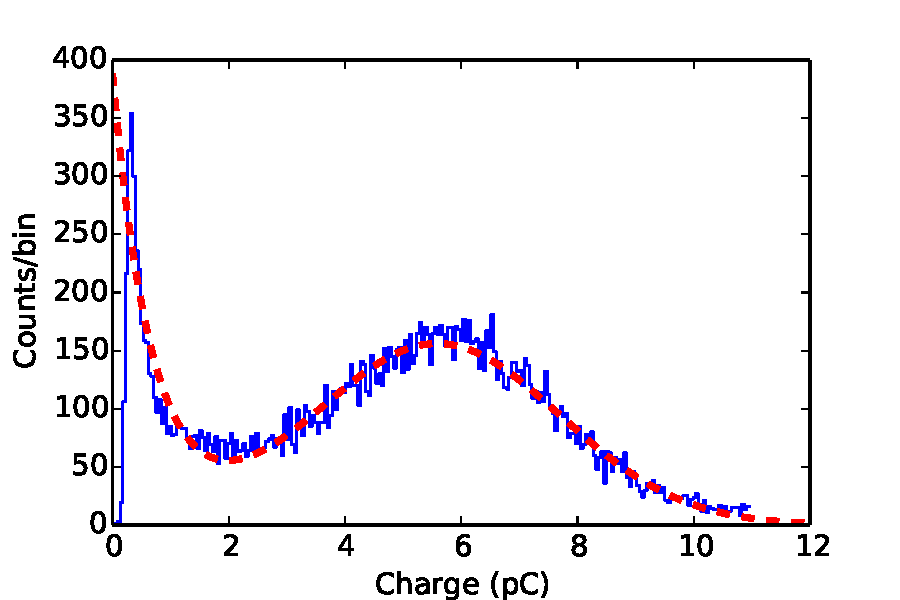
\includegraphics[width=0.6\textwidth]{graphics/dom/domcal/hvfit.pdf}
 \caption{Sample SPE charge spectrum as recorded by DOMCal and fit
   \textit{in situ} with a Gaussian+exponential model.} 
 \label{fig:domcal_hvfit}
\end{figure}

% From JK DOMCal HV Settings.ipynb
\begin{figure}[!h]
 \centering
 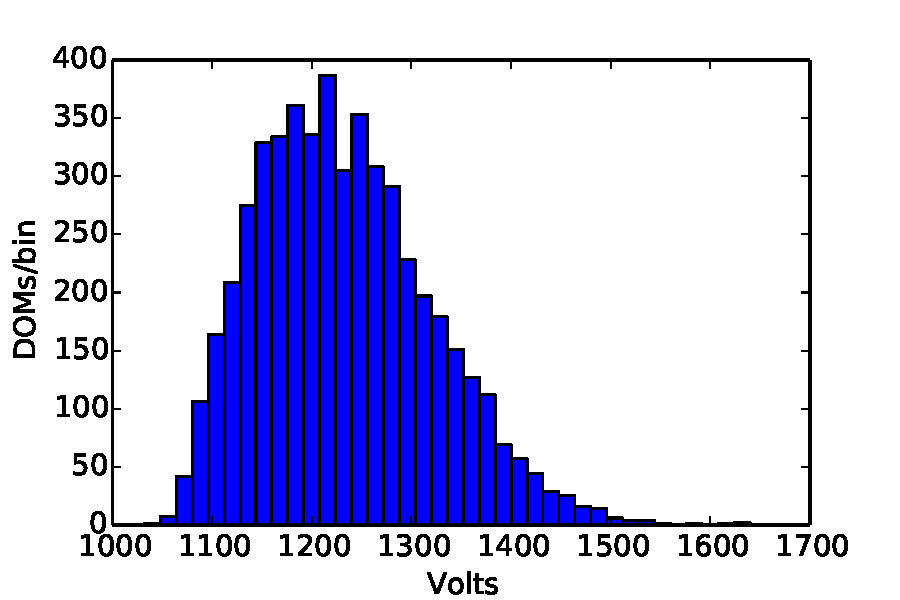
\includegraphics[width=0.6\textwidth]{graphics/dom/domcal/inice_hv_2016.pdf}
 \caption{PMT high voltage at $10^7$ gain for in-ice DOMs.}
 \label{fig:domcal_hv_settings}
\end{figure}

\subsection{\label{sec:waveformcal}Waveform Calibration}

An ATWD waveform consists of readouts from 128 effectively independent
digitizers, while an fADC waveform consists of successive outputs of a 6-stage
pipelined digitizer (256 samples). Two calibration constants per digitizer are needed to turn each of these
raw readout values (an integral number of ADC counts) into a
voltage, from which the deposited charge is calculated. The deposited
charge is the basis for all energy measurements in IceCube. The
calibration constants needed are 1) the pedestal, the value the digitizer reads when the input voltage is zero, and
2) the gain, the input voltage required to increase the readout value by one count. 

Since each bin of each ATWD channel is read from an independent
digitizer, it is important to distinguish between the pedestals of
individual bins and the common pedestal of the entire waveform. The
baseline is the mean of the pedestals of each bin in a waveform. For
the fADC, this is the same as the pedestal. The pedestal pattern is
the deviation of each bin's pedestal from the common baseline. For the
fADC, this is identically zero. Since 2008, the DOM has subtracted the
pedestal pattern from
the ATWD waveform before sending it to the surface. The pedestal pattern is computed at the beginning of each
run by comparing 25 averaged pedestals. The autocorrelation coefficient
of the difference between pairs of averaged pedestals is computed to detect light
contamination in the pedestals, and the shift between the baseline of
the pairs is calculated to determine that the baseline is stable. This
procedure ensures that fewer than 1 DOM in 1000 runs will contain a
contaminated baseline. Thereafter, both ATWD
and fADC waveforms can be calibrated by first subtracting the common
baseline from each bin, then multiplying by the gain. Correct
measurement of the common baseline is critical to correct charge
measurement and energy reconstruction.

The baseline is set to about 10\% of the maximum value of the
digitizer counts in
order to capture signals that go below the baseline. Since 2012, the
baseline value is set by the DAQ configuration in order to ensure 
stability. The baseline value differs for each digitizer channel in
each DOM, ranging from 112 to 161 counts in the fADC and 109 to 172
counts in the ATWD. The baselines for each digitizer channel in each DOM are measured with
beacon hits, forced triggers which are collected at a rate of 1.2~Hz
per DOM
in in-ice DOMs and 4.8~Hz in IceTop DOMs. Beacon waveforms
from the fADC and ATWD of a typical DOM are shown in Figure~\ref{fig:raw_baselines}.

\begin{figure}[!h]
  \captionsetup[subfigure]{labelformat=empty}
  \centering
  \subfloat[]{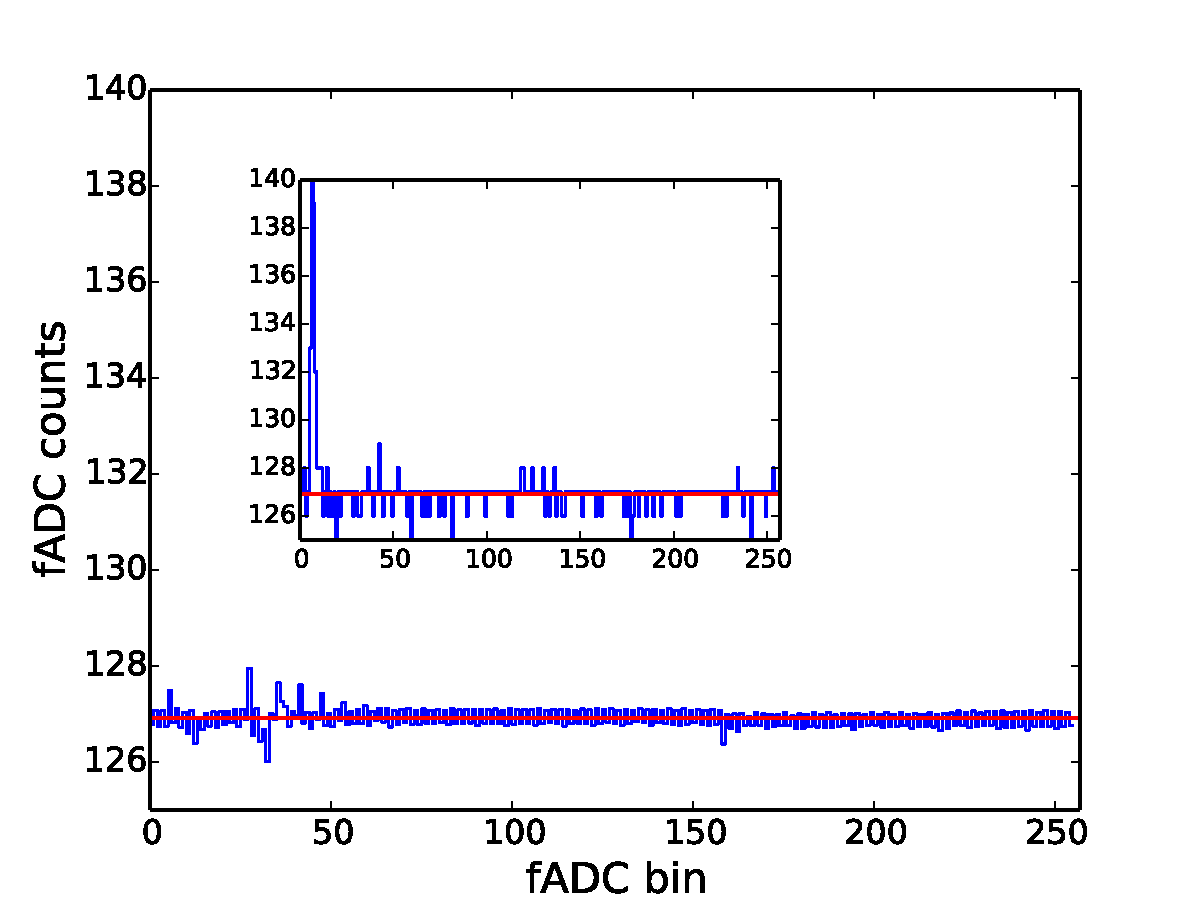
\includegraphics[width=0.5\textwidth]{graphics/dom/reliability/fadc_average_beacon_raw.pdf}}
  \subfloat[]{\includegraphics[width=0.5\textwidth]{graphics/dom/reliability/ATWD_average_beacon_raw.pdf}}
  \caption{Beacon waveforms from the fADC (left) and ATWD (right) of
    an IceCube DOM. The waveforms are an average of $\sim1000$ beacon
   launches. The baseline, which is the mean value of the
    beacon waveform, is shown as a horizontal red line. Typical raw SPE
    waveforms are inset.}
  \label{fig:raw_baselines}
\end{figure}

The digitizer gain is measured by DOMCal (Sec.~\ref{sec:domcal}), a single
value for the fADC waveform and a bin-dependent value for the ATWD
waveform. The calibrated waveform voltage is then

\begin{equation}
  \mathrm{voltage} = \mathrm{(counts - baseline) \times gain}
\end{equation}

The waveform start time is then corrected for the PMT transit time,
the average time it takes a pulse to propagate through the entire
PMT and Delay Board. The PMT transit time correction $t_{\mathrm{transit}}$ is
dependent on the PMT high voltage $V$:

\begin{equation}
  t_{\mathrm{transit}} = \frac{m}{\sqrt{V}} + b
\end{equation}

\noindent where $m$ and $b$ are determined by DOMCal. The typical value of $m$
is 2000~ns$\cdot \sqrt{\mathrm{V}}$, and the typical value of $b$ is
80~ns, which includes the 75~ns delay line of the Main Board. The
typical transit time is therefore 130~ns.  Waveform start times from the
second ATWD chip and the fADC are further 
corrected for the delay $\Delta t$ with respect to the first ATWD
chip, so the total start time correction is $t_{\mathrm{transit}} + \Delta t$.

Finally, the waveforms are corrected for the effects of droop from the
transformer that couples the Main Board to the PMT output. The toroid
coupling effectively acts as a high-pass filter on the PMT output
that makes the tails of the waveforms ``droop'' and even
undershoot the baseline. This effect is temperature-dependent and is larger
at lower temperatures. The droop correction inverts the effect of the high-pass
filter and eliminates the undershoot in the waveform tails. This is
done by calculating the expected reaction voltage from the toroid at
each time, and adding the reaction voltage to the calibrated waveform
to compensate. The reaction voltages decay exponentially
according to a temperature-dependent model of the transformer behavior. 
When a readout contains consecutive launches from the same
DOM, the reaction voltages at the end of the last launch are used to
correct for the residual droop in the follow-on launch.  DOMs
use two types of toroid transformers: the ``old toroid'' with a short
time constant that was used in early DOM production, and a ``new
toroid'' with a longer time constant that produces less
distortion.  The full correction is modeled with a dual time constant,
where the DOM's transient response $\tilde{\delta}(t)$ to an input
signal $\delta(t)$ is given by

\begin{equation}
\tilde{\delta}(t) = \delta (t) - N((1 - f) e^{t/\tau_1} +f
e^{t/\tau_2})
\end{equation}

\noindent The first time constant $\tau_1$ is given by 

\begin{equation}
\tau_1(T) = A + \frac{B}{1 + e^{(-T/C)}}
\end{equation}

\noindent where $T$ is temperature and $A$, $B$, $C$, $N$ and $f$ are determined empirically.
For old toroid DOMs, the second time constant $\tau_2 =0.75\tau_1$. For new
toroid DOMs, $\tau_2$ is 500~ns.

\subsection{\label{sect:dom:rapcal}RAPCal}

The Reciprocal Active Pulsing calibration (RAPCal) is a
continuously running method for translating hit timestamps from the the
individual free-running DOM clock domains to the clock domain in the
ICL, which is synchronized to UTC
(Sec.~\ref{sect:online:master_clock}). While data transmission is paused, a
bipolar pulse is generated and sent to each DOM over the power/communications wire pair.  After
this pulse has been received, a bipolar pulse --- having the same shape
as the one generated on the surface --- is generated in the DOM and sent
back to the surface.  The bipolar pulses are time stamped by the local
clock at each transmission and reception point.  The symmetry of the
pulses sent in each direction and symmetry of the down- and up- cable
transmission enables a translation from each free-running DOM clock to the surface clock and hence to UTC, without prior knowledge of the cable length or its dispersive properties. The base implementation is described in \cite{ICECUBE:DAQ}; we describe here the details of the time translation algorithm and validation of the DOM relative time calibration.

\begin{figure}[!h]
 \centering
 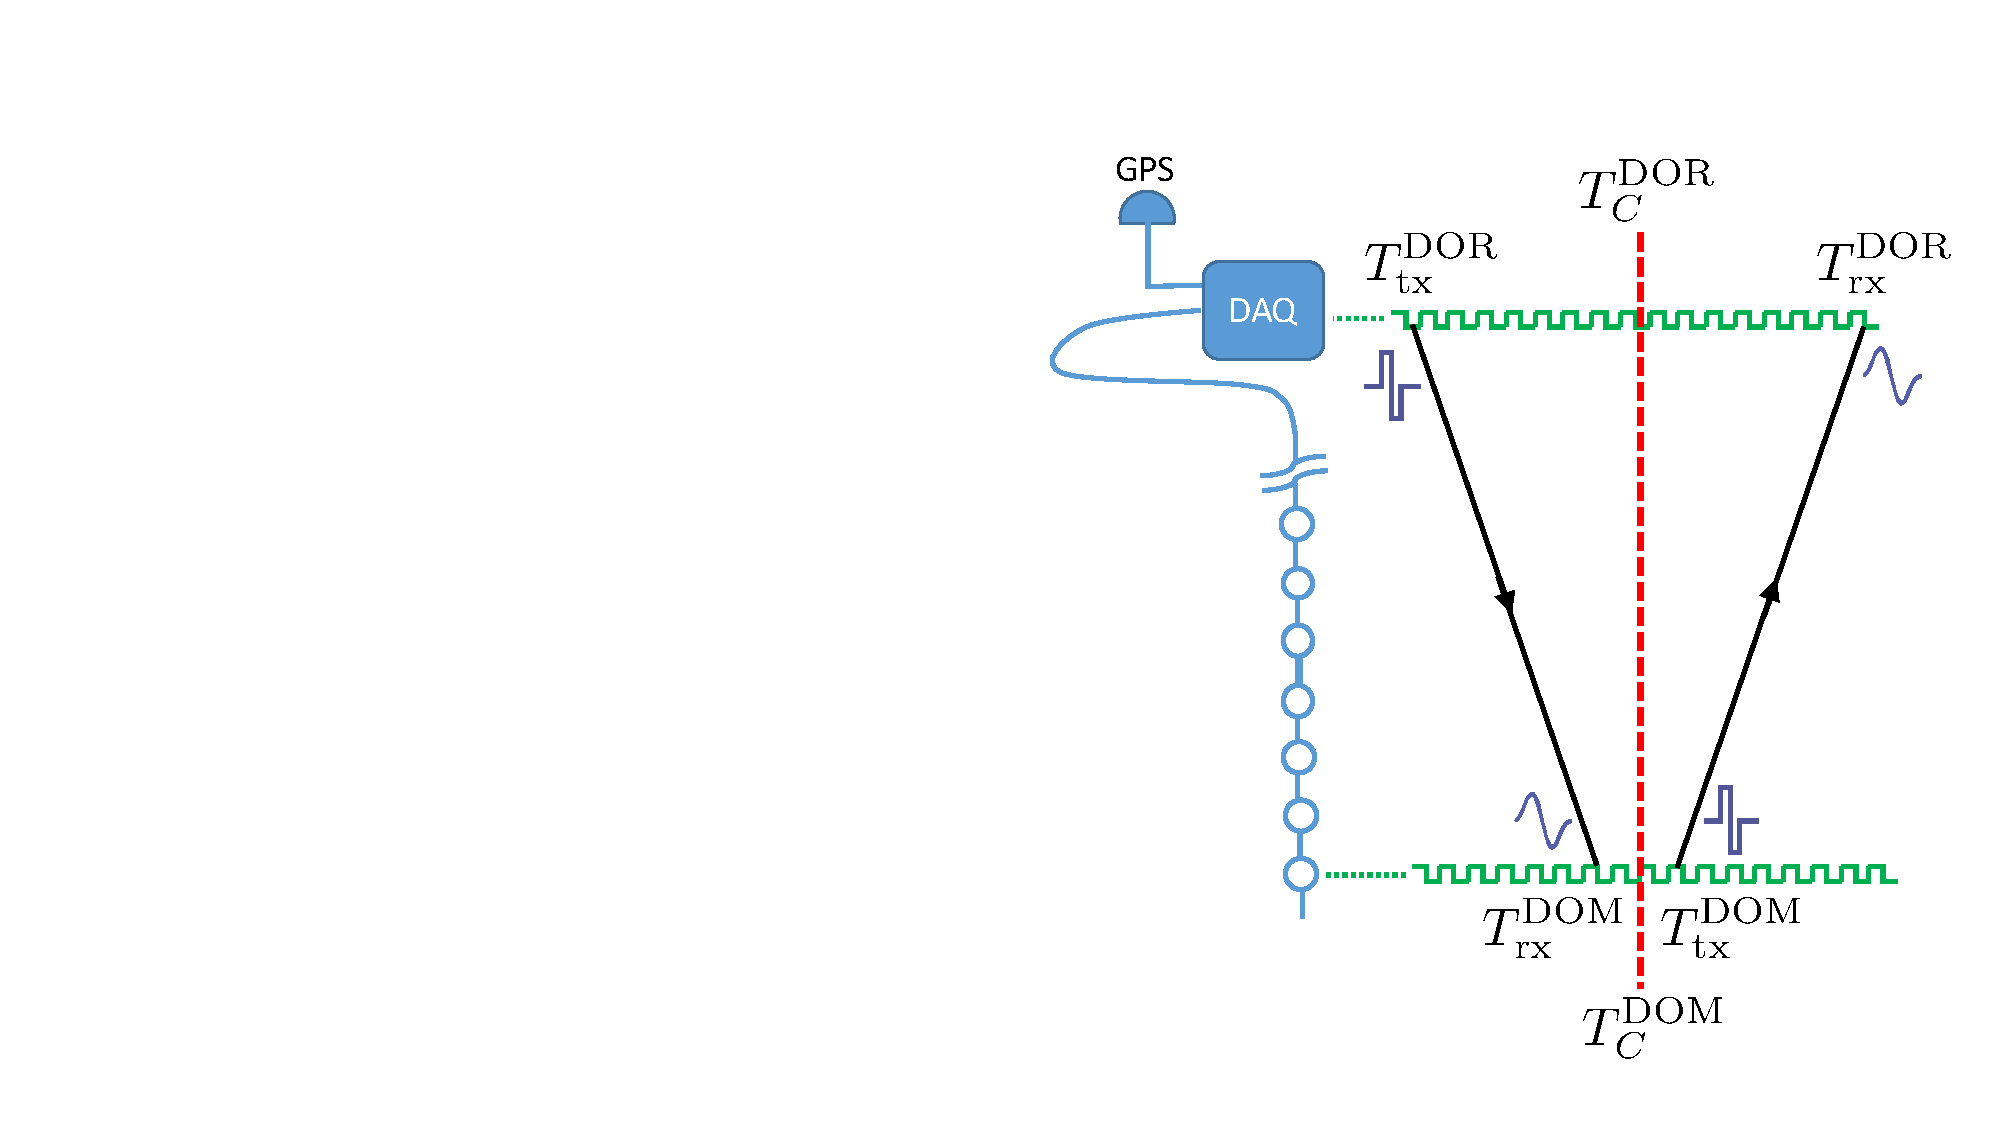
\includegraphics[width=0.6\textwidth]{graphics/dom/rapcal/rapcal_symmetry.pdf}
 \caption{Diagram of the RAPCal time calibration scheme.
   Each transmitted and received pair of signals is
   timestamped in the local clock domain, and by the symmetry of the
   situation the midpoints are synchronous.}
 \label{fig:rapcal_symmetry}
\end{figure}

\begin{figure}[h]
 \centering
 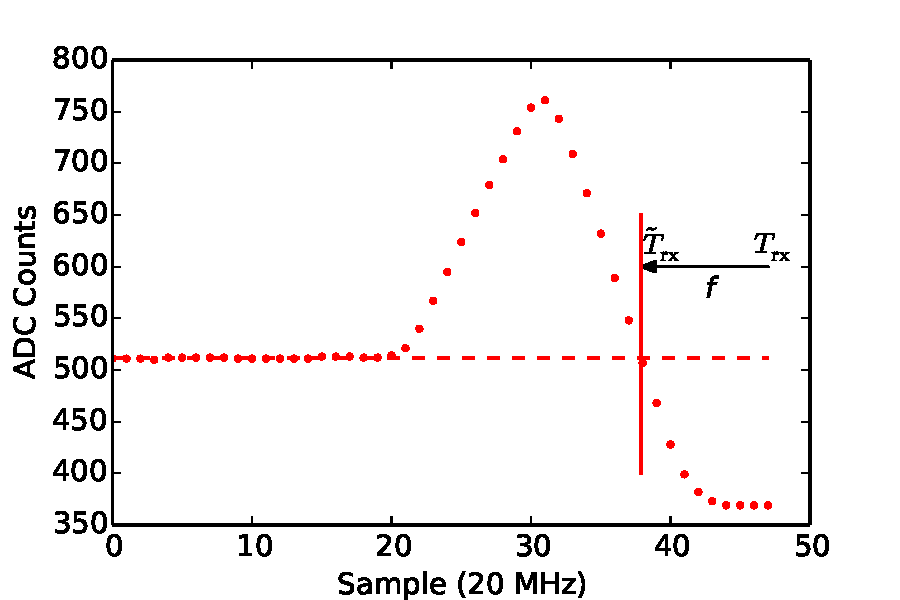
\includegraphics[width=0.6\textwidth]{graphics/dom/rapcal/dom_wf_zero_crossing.pdf}
 \caption{Digitized RAPCal pulse as received by a DOM, after cable dispersion.  The
   zero-crossing of the baseline-subtracted pulse is used as a fine-delay
   correction to the received timestamp.}
 \label{fig:rapcal_zero_crossing}
\end{figure}

A RAPCal pulse sequence to each DOM results in a series of four timestamps
$T_{\mathrm{tx}}^{\mathrm{DOR}}$, $T_{\mathrm{rx}}^{\mathrm{DOM}}$, 
$T_{\mathrm{tx}}^{\mathrm{DOM}}$,  and $T_{\mathrm{rx}}^{\mathrm{DOR}}$
(Fig.~\ref{fig:rapcal_symmetry}), with timestamps in 20 MHz units
of the DOM and surface (DOR, see Sect.~\ref{sect:online:master_clock}) clocks.  The received dispersed bipolar pulses
are digitized by the communications ADCs and 
timestamped.  A ``fine delay'' correction $f$ to
$T_{\mathrm{rx}}^{\mathrm{DOM}}$ and $T_{\mathrm{rx}}^{\mathrm{DOR}}$ is calculated by interpolating
to find the negative-going zero crossing, relative to a baseline voltage
calculated using the initial samples of the waveform (Fig.~\ref{fig:rapcal_zero_crossing}):

\begin{equation}
  \tilde{T}_{\mathrm{rx}} = T_{\mathrm{rx}} - f\ .
\end{equation}


\noindent The midpoints $T_C^{\mathrm{DOR,DOM}}$ halfway between $T_\mathrm{tx}^{\mathrm{DOR,DOM}}$ and
$\tilde{T}_\mathrm{rx}^{\mathrm{DOR,DOM}}$ are identified as synchronous.
To translate an arbitrary DOM timestamp $t$ to UTC
time, we use the RAPCal results bracketing $t$ to derive a linear
relationship

\begin{equation}
  \mathrm{UTC}(t) = (1+\epsilon)(t - T_C^{\mathrm{DOM}}) +
  T_C^{\mathrm{DOR}} + \Delta\ .
\end{equation}

\noindent The slope $(1+\epsilon)$ accounts for drifts in the 20 MHz DOM
clocks and is calculated from the midpoints $T_C$ of the bracketing RAPCal
results: 

\begin{equation}
  1+\epsilon = \frac{T_{C,2}^{\mathrm{DOR}} -
    T_{C,1}^{\mathrm{DOR}}}{T_{C,2}^{\mathrm{DOM}} -
    T_{C,1}^{\mathrm{DOM}}}\ .
\end{equation}

\noindent The median magnitude of $\epsilon$ is $1.34 \times 10^{-6}$.
Finally, because the timestamps $T^{\mathrm{DOR}}$ count the offset into 
the current UTC second, the UTC time offset $\Delta$ of the previous
1-second boundary, provided by the master clock, is added.

The stability and repeatability of the calibration is monitored by
tracking the cable delay from multiple measurements, defined as

\begin{equation}
  T_{\mathrm{cable}} = \frac{1}{2} \left( ( T_{\mathrm{rx}}^{\mathrm{DOR}} -
  T_{\mathrm{tx}}^{\mathrm{DOR}} ) - (1+\epsilon)(T_{\mathrm{tx}}^{\mathrm{DOM}} -
  T_{\mathrm{rx}}^{\mathrm{DOM}} )\right) \ .
\end{equation}

\noindent A representative distribution of $T_{\mathrm{cable}}$ from one DOM over an 8-hour
data-taking run is shown in Fig.~\ref{fig:rapcal_cable_len}, with a
standard deviation of 0.6 ns. In typical operating conditions, a RAPCal procedure
is repeated once per second for each DOM.  Individual $T_{\mathrm{cable}}$
measurements that deviate by more than 10 ns from a moving average are discarded.

\begin{figure}[!h]
 \centering
 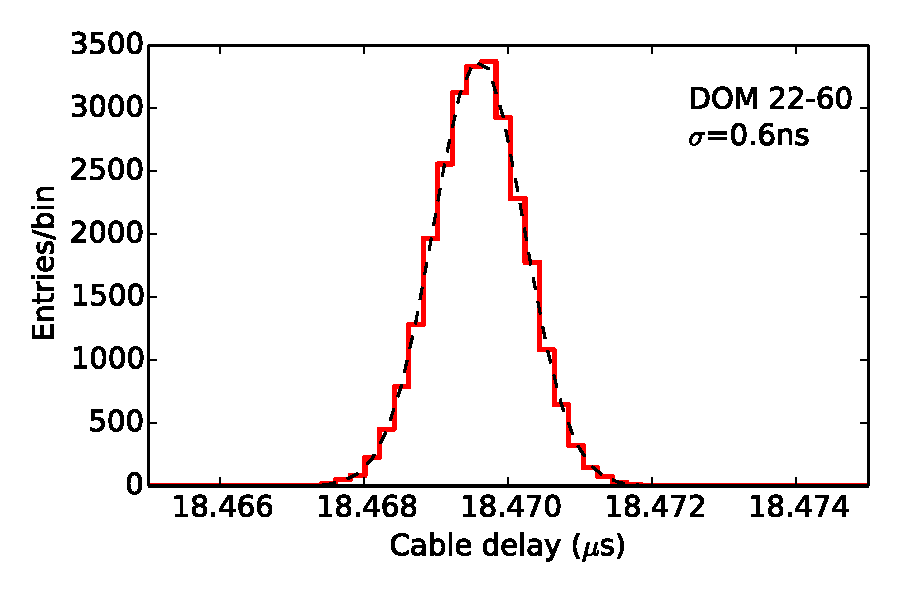
\includegraphics[width=0.6\textwidth]{graphics/dom/rapcal/tcal_hist_22-60.pdf}
 \caption{Distribution of one-way cable delays from multiple RAPCal
   measurements on DOM 22-60 (bottom of String 22).}
 \label{fig:rapcal_cable_len}
\end{figure}

The time calibration through the entire data acquisition and software
processing chain is verified using the LED flashers. During
commissioning, performed on each string after deployment, all 12~LEDs on each DOM are flashed simultaneously at
maximum brightness, and the arrival times of the first photons at the DOM above the flashing DOM
are recorded. Given the vertical spacing of 17~m on a standard IceCube
string and the group index of
refraction of  1.356 in ice at 400~nm \cite{price_woschnagg_ice}, the expected light travel time
from the flashing DOM to the DOM above is 77~ns. In DeepCore, the DOM
vertical spacings are 10~m and 7~m, corresponding to light travel
times of 45~ns and 32~ns respectively. The mean light travel
time to the DOM above for all flashing DOMs in ice is shown in
Fig.~\ref{fig:flashertiming}. The mean arrival time agrees with the
expectation for the DeepCore DOMs. For the standard DOMs, the observed
light travel time is about 3~ns longer than the expected light travel
time, due to the effects of scattering in the ice over the longer distance. Muons are also used to
verify the time calibration, including the absolute time difference
between the IceTop surface stations and the in-ice DOMs~\cite{IC3:perf}.

\begin{figure}[!h]
  \captionsetup[subfigure]{labelformat=empty}
  \centering
  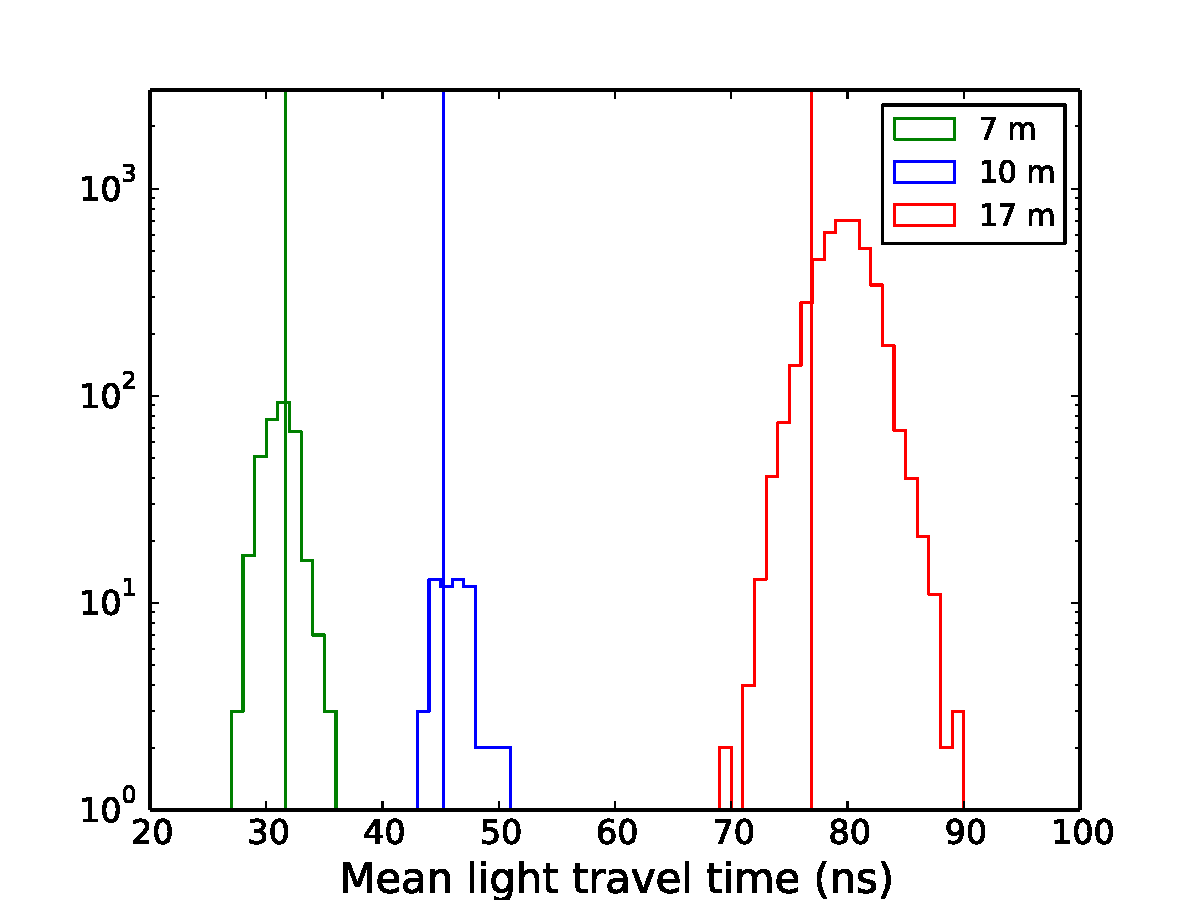
\includegraphics[width=0.8\textwidth]{graphics/dom/rapcal/flashmean.pdf}
  \caption{Time from flasher emission to detection at the DOM above for 17~m vertical spacing
    (red), 10~m vertical spacing (blue) and 7~m vertical spacing
    (green). The expected light travel times in ice for each distance are marked with
    vertical lines.}
  \label{fig:flashertiming}
\end{figure}

\subsection{\label{sec:domeff}DOM Optical Efficiency}

A baseline value for the photon detection efficiency has been established
by combining PMT measurements at 337~nm and a separate model of wavelength-
and angle-dependent effects.  Absolute sensitivity measurements were
performed on 13 IceCube PMTs, using photons that were Rayleigh scattered by
90$^{\circ}$ from a primary 337~nm laser beam of known
intensity~\cite{ICECUBE:PMT}. The results agree well with independent
Hamamatsu measurements of sensitivity in the range $270-730$nm, which
were then normalized to the 337~nm measurement.  The resulting quantum
efficiency at the center of the PMT and at 390~nm is 25\%.  A full
simulation model for the DOM includes the wavelength dependence of the PMT
response, optical absorption in the DOM glass and gel, discriminator
threshold effects, and photocathode non-uniformity.  The angular dependence is
dominated by the shape of the photocathode and its response variation away
from the center, which was measured for 135 PMTs~\cite{ICECUBE:PMT}.

The laboratory-based efficiency model was supplemented with \textit{in
  situ} measurements using Cherenkov light from muons in the ice. The
efficiency measured \textit{in situ} includes effects of the cable
shadowing the DOM and the refrozen ``hole ice'' in the vicinity of the
DOM. In one
study, low-energy muons (median energy 82~GeV) with well-understood light
emission were selected to illuminate the downward-facing PMTs in the ice as
directly as possible. The number of photons detected at different
distances from these muons was then compared to predictions of the
simulation model~\cite{IC3:ereco}.  Based on this and other \textit{in
  situ} analyses, the central value for the efficiency was adjusted upward
by 10\% in the simulation, compared to the baseline.  For physics analyses,
DOM efficiency is generally included as a nuisance parameter with prior
uncertainty of 10\% that includes other uncertainties related to
generation and propagation of the light. Additional laboratory measurements
on assembled DOMs are in progress, including wavelength- and angle-dependent
effects, and are expected to reduce uncertainties~\cite{ICECUBE:DOMEFF}.

The absolute calibration at 337~nm was performed at room temperature on a
small subset of IceCube PMTs. The relative efficiency of all assembled DOMs
was separately measured as part of production testing
(Sec.~\ref{sec:dom_prodtest}), using a 405~nm pulsed laser and a system of
fibers and diffusers to illuminate DOMs evenly within 50$^{\circ}$ of the
optical axis.  Using this system, the relative efficiency of DeepCore DOMs
(high quantum efficiency type) was measured to be higher by a factor
of 1.39
compared to standard IceCube DOMs, agreeing well with the
manufacturer-specified value of 1.40. Further \textit{in situ} studies
using muons yielded a factor of 1.35~\cite{ICECUBE:DC}, an
effective value including the Cherenkov spectrum folded with the different
wavelength sensitivity curves of the two types of PMTs.  The production
testing system also established that the efficiency change from room
temperature to $-40^{\circ}$~C is less than 1\% when gain is maintained at
the design value of $10^7$.

\subsection{\label{sec:baselines}Baseline Voltage Stability}

The beacon hits from which the digitizer baselines are derived are
monitored continuously throughout the year. The average values of the
beacon baselines are very stable, with shifts of no more than
0.2~counts year to year, corresponding to 0.018~mV in the fADC and
0.025~mV in the high-gain ATWD channel. The single photoelectron
charge peak is stable to within 0.05~PE. The baseline shifts from May
2015 to April 2016 are shown in Fig.~\ref{fig:baseline_stability_2015}. 

\begin{figure}[!h]
 \centering
 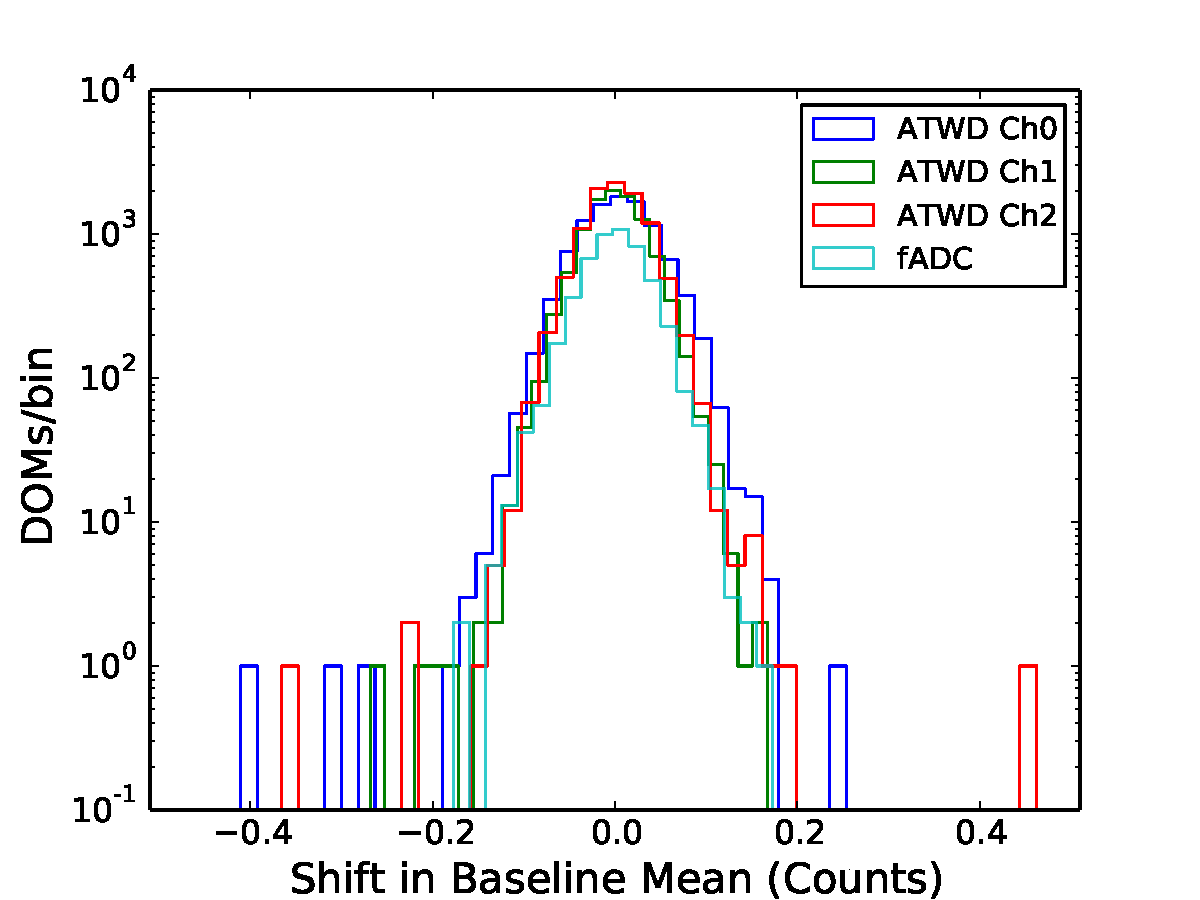
\includegraphics[width=0.6\textwidth]{graphics/dom/reliability/baseline_stability_2015.pdf}
 \caption{Distribution of shifts in baseline values in all ATWD
   channels and the fADC for all DOMs from May 2015 to April
   2016. The DOM configuration was unchanged during this period.}
 \label{fig:baseline_stability_2015}
\end{figure}

Every year when the detector
is recalibrated, adjustments in the SPE discriminator threshold can
cause shifts of up to 0.6~counts (0.54~mV) in the fADC
baselines. ATWD baselines are unaffected by the SPE discriminator
setting. Correcting recorded waveforms for the effect of transformer
coupling as described in Sec.~\ref{sec:waveformcal} has
the side effect that small DC offset errors are converted into
apparent PMT current that increases linearly in time over the course
of a few microseconds. The effect is stronger for DOMs with old-type toroid
transformers, where a baseline error of 0.6~counts can 
turn an actual deposited charge of 1~PE into a measured charge of over
2~PE with an unphysical time structure. The observed distortion in a
simulated single photoelectron charge due to fADC baseline shifts is
shown in Figure~\ref{fig:charge_fadcshift}.  To avoid this problem, whenever the
discriminator thresholds are changed, the fADC baselines are re-measured,
and the values used for calibration are updated. As long as 
the discriminator thresholds are unchanged, the baselines are stable
to within 0.2~counts
as shown above, and no charge distortion is seen at that level of
baseline stability.

\begin{figure}[!h]
 \centering
 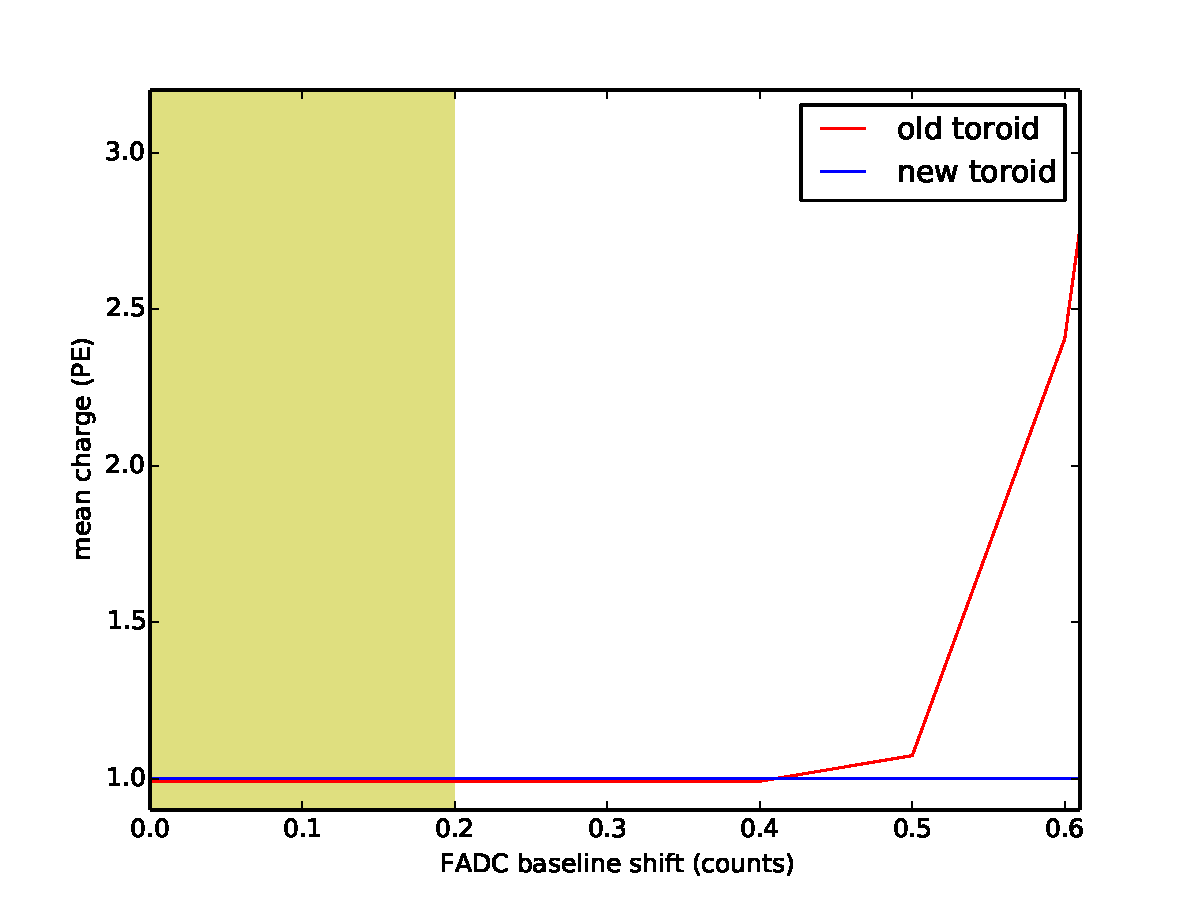
\includegraphics[width=0.8\textwidth]{graphics/dom/reliability/charge_fadcshift.pdf}
 \caption{Reconstructed charge from a simulated single photoelectron
   deposit as a function of fADC baseline shift, for both old- and
   new-toroid DOMs. The shaded region indicates the observed range of 
   baseline variation from the nominal value in ice; no observable
   distortion in the charge spectrum is seen at these values.}
 \label{fig:charge_fadcshift}
\end{figure}

The baselines are sensitive to radio frequency interference (RFI). In
2009, RF signals from the COBRA meteor radar transmitter broadcasting at
46.3~MHz \cite{meteor_radar}
appeared as sinusoidal or spiky signatures in the waveform
baselines.  To mitigate this effect, one DOM was operated without PMT high
voltage and used to monitor the RF broadcasts and tag periods of RFI in
order to avoid data contamination.  Also
in 2009, DOM 68-42 was damaged by a high voltage setting during DOM
calibration, and appeared to begin sparking, causing sinusoidal waveforms
to appear in the baselines of neighboring DOMs. The meteor radar
transmitter is no longer operating, and investigations into RFI
from more recent radar activities at South Pole (SuperDARN
\cite{superdarn}) have revealed no measurable interference, either in DOM
baselines or in RAPCal time stability. 

\subsection{\label{sec:gain_stability}Gain Stability}

The gain stability of the DOM, or the stability of the amplified charge
from converted photons, depends on a number of factors including stability
of the PMT high voltage, Main Board channel amplifiers, and the digitizers.
We can examine these subsystems using both historical calibration results
as well as by tracking the SPE charge during data-taking.

The gain stability of the DOM electronics includes variations in the
front-end electronic amplifiers and the digitizers themselves.  The
stability is checked by comparing the Main Board channel amplifier gains
from sets of calibrations taken from 2011 to 2016
(Fig.~\ref{fig:domcal_ch_gain}).  From year to year, the amplifier gain 
calibration is repeatable to 0.1\%, 0.2\%, and 0.5\% in the high-gain,
medium-gain, and low-gain channels respectively.  Since detector completion
in 2011, a small systematic shift of $-0.3\%$ is visible in the low-gain
channel, but this is corrected by updating the calibration constants of
each DOM.

% JK: DOMCal Channel Gain Stability.ipynb
\begin{figure}[!h]
  \captionsetup[subfigure]{labelformat=empty}
  \centering
  \subfloat[]{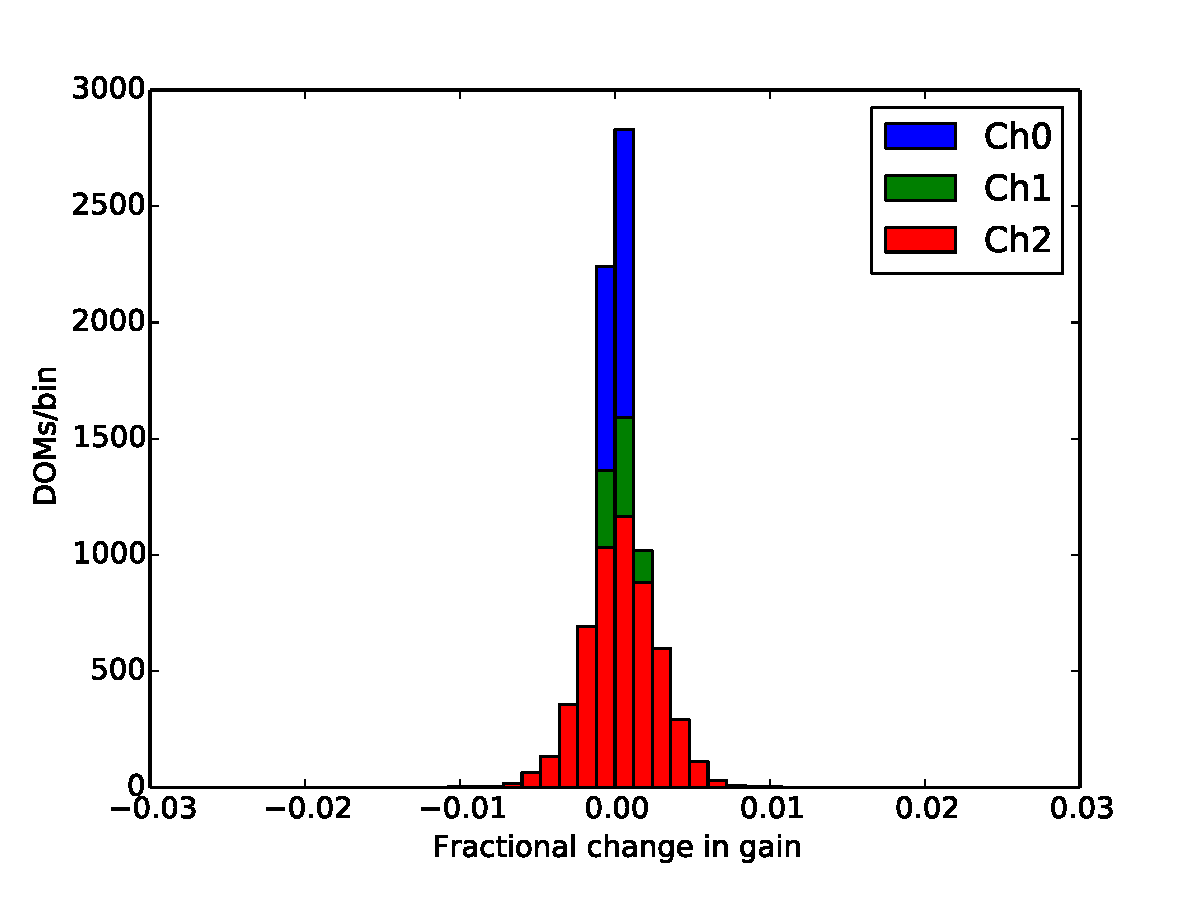
\includegraphics[width=0.5\textwidth]{graphics/dom/reliability/channel_gain_shift_2016_2015.pdf}}
  \subfloat[]{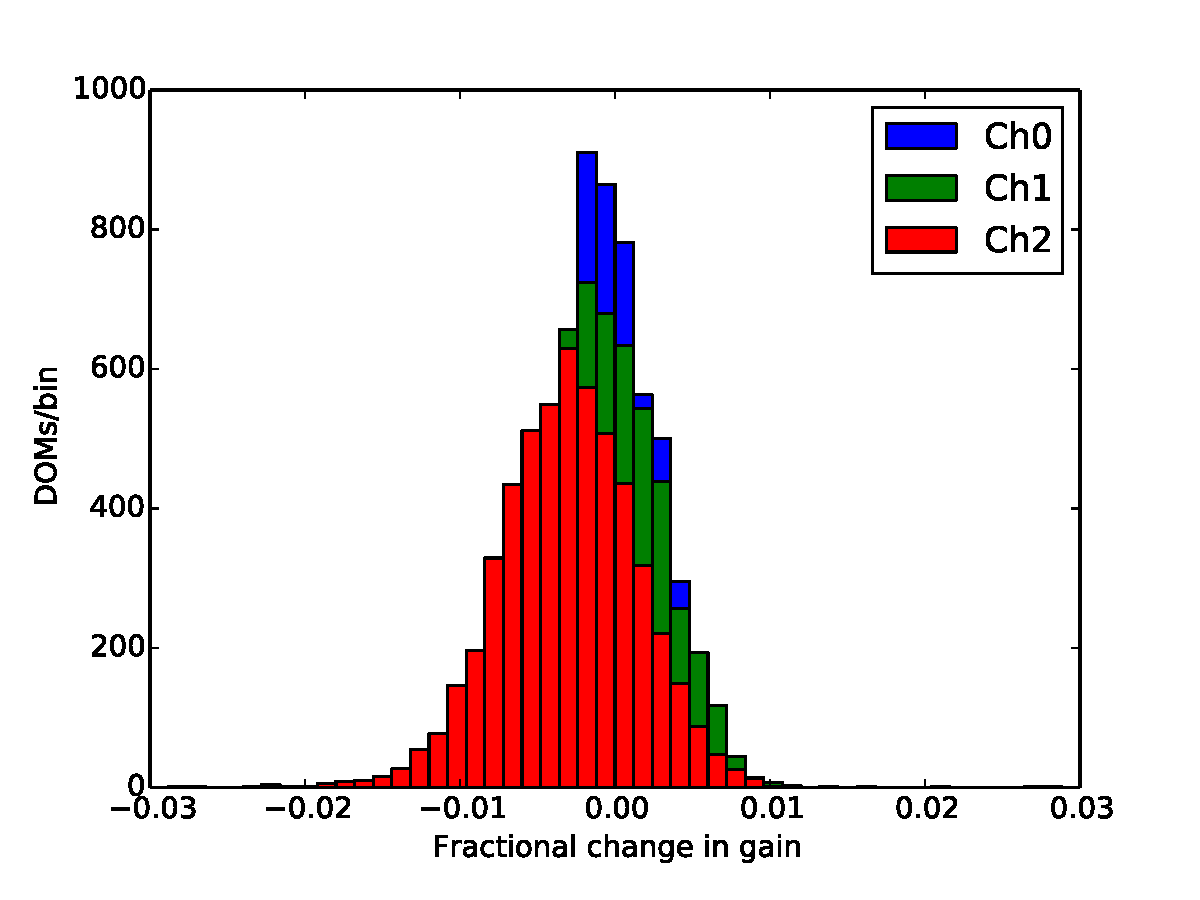
\includegraphics[width=0.5\textwidth]{graphics/dom/reliability/channel_gain_shift_2016_2011.pdf}}
  \caption{Fractional DOM channel amplifier gain shifts, from 2015 to
    2016 (left) and 2011 to 2016 (right).  Channels 0, 1, and 2 are
    high gain, medium gain, and low gain respectively.}
  \label{fig:domcal_ch_gain}
\end{figure}

The PMT gain stability is monitored during data-taking using the
single photoelectron peak of the charge distribution on each DOM from
cosmic ray muons. A
Gaussian + exponential function is fit to the peak region as in
Fig.~\ref{fig:spe_fit_thresh}, and the mean of the Gaussian is
tracked throughout the year. The threshold, defined as the bin in the histogram for which 99\% of the area of the histogram is contained in the sum of all higher bins, is also tracked through
the year. The peak position is calibrated to 1~PE
and is stable to within 0.01~PE for 95\% of all DOMs, as shown in
Fig.~\ref{fig:gain_spe_stability}. Over 99\% of DOMs show no
measurable change in the threshold as long as the discriminator
thresholds are unchanged; these settings are only changed once per year.

\begin{figure}[!h]
 \centering
 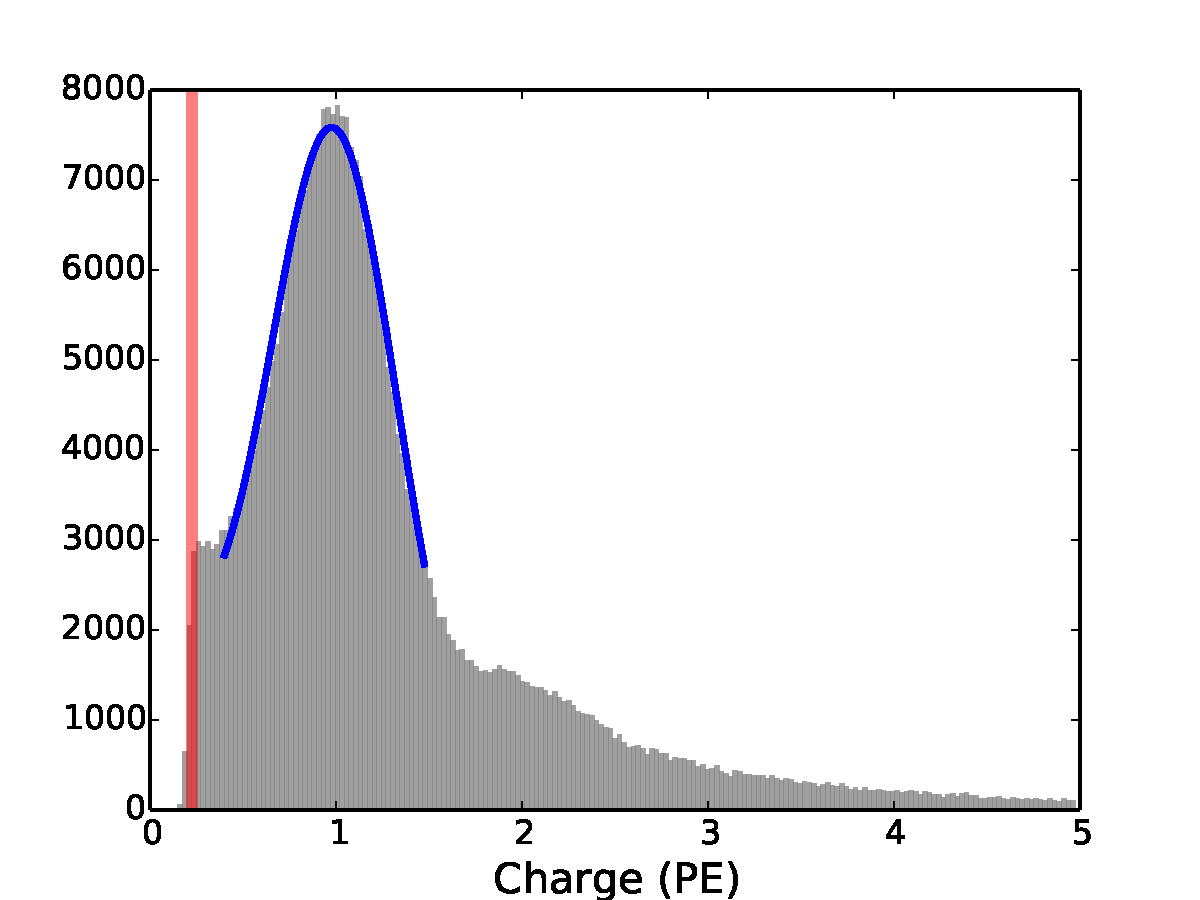
\includegraphics[width=0.6\textwidth]{graphics/dom/reliability/chargedist.pdf}
 \caption{Charge distribution of a typical in-ice DOM. The threshold
   is marked in red, and a Gaussian + exponential fit to
   the SPE region is shown in blue. The mean of the Gaussian is used
   to monitor the gain stability.}
 \label{fig:spe_fit_thresh}
\end{figure}

\begin{figure}[!h]
  \captionsetup[subfigure]{labelformat=empty}
  \centering
  \subfloat[]{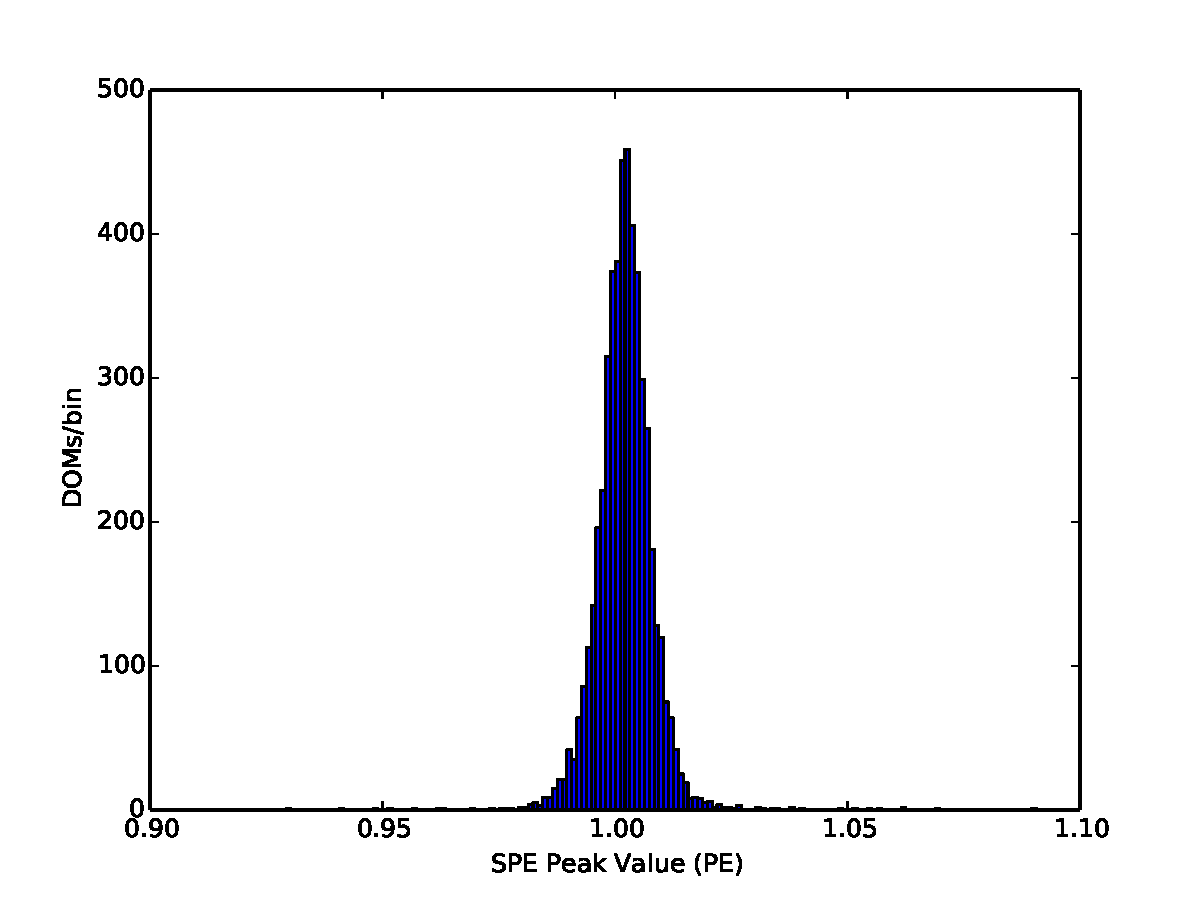
\includegraphics[width=0.5\textwidth]{graphics/dom/reliability/mean_value_2015.pdf}}
  \subfloat[]{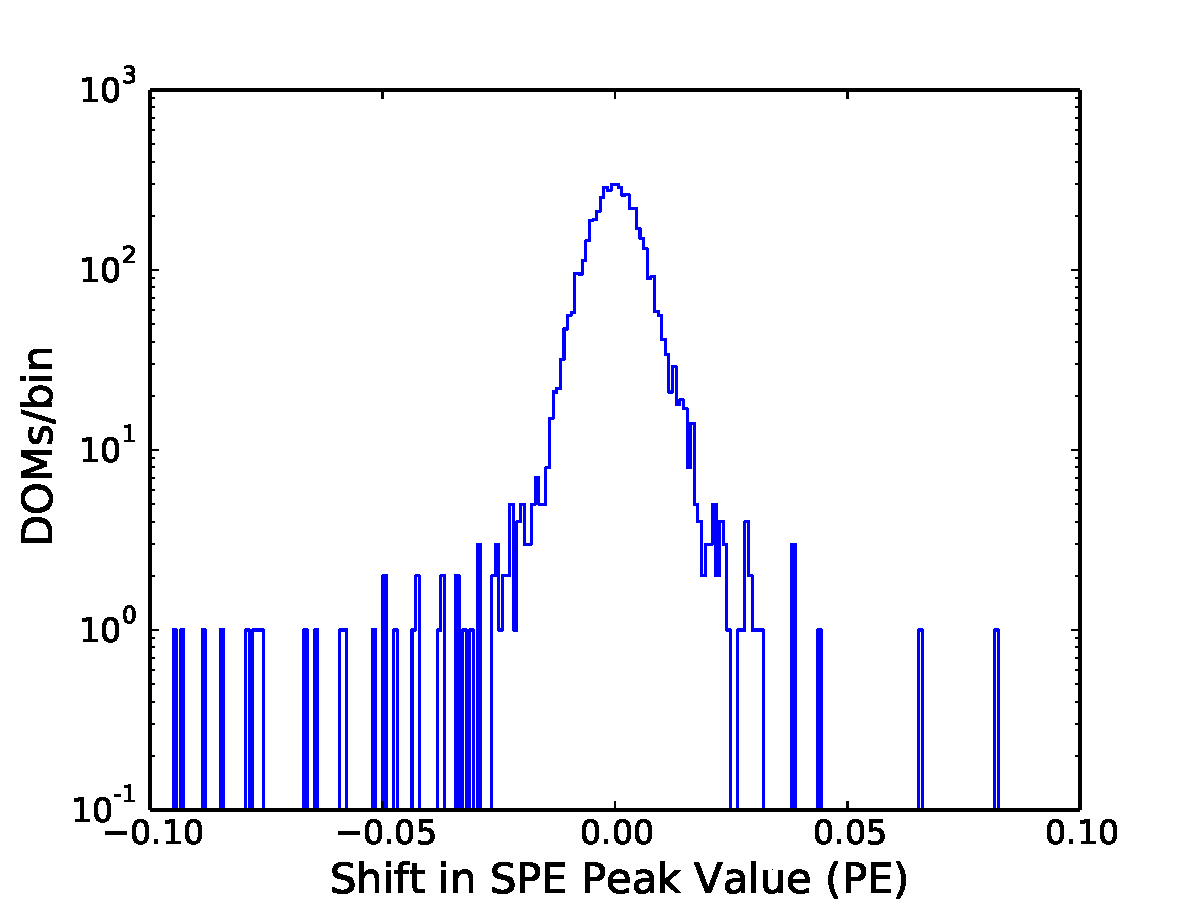
\includegraphics[width=0.5\textwidth]{graphics/dom/reliability/meandiff_2015.pdf}}
  \caption{Distribution of the mean of the Gaussian fit to the SPE
    peak (left) and the shift in this value in every in-ice DOM between  May 2015 and April
   2016.}
  \label{fig:gain_spe_stability}
\end{figure} 

There are on the order of 12~DOMs that show unpredictable, abrupt shifts in the SPE peak
position of 0.05~PE or more. Fig.~\ref{fig:gainshift_spe} shows the time history of the
SPE peak position of one of these DOMs over 4~months. The peak shift
corresponds to increases or decreases in the multi-photoelectron (MPE) scaler rate,
indicating that the SPE peak shift is indeed caused by a change in the DOM
gain. However, the SPE scaler rate is stable, indicating that the
probability to detect single photons is effectively unchanged.

\begin{figure}[!h]
 \centering
 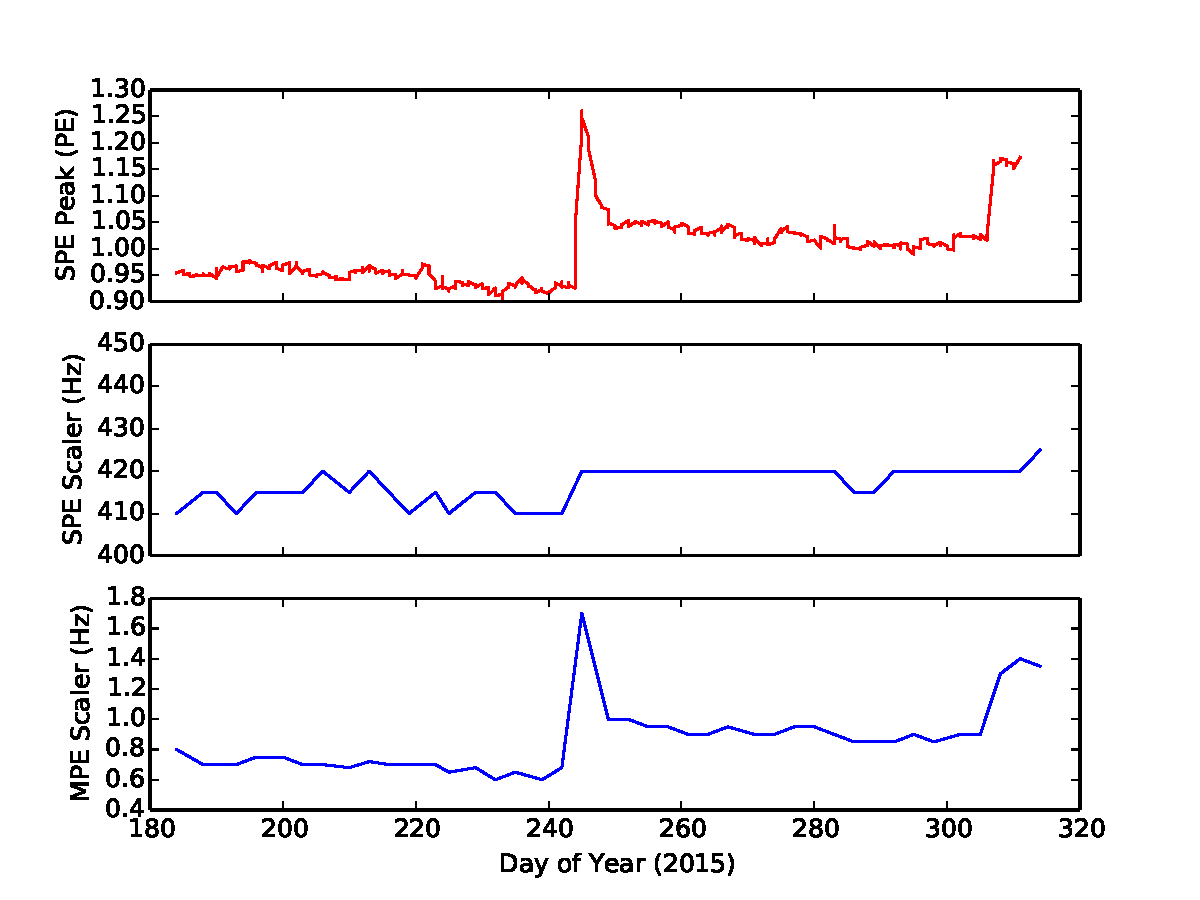
\includegraphics[width=0.8\textwidth]{graphics/dom/reliability/gainshift.pdf}
 \caption{Mean of the Gaussian fit to the SPE peak (top) and the SPE
   scaler rate (middle) and MPE
   scaler rate (bottom) from July 2015 to November 2015 for a DOM
   which shows unpredictable gain shift behavior. The DOM
   configuration was unchanged during this period.}
 \label{fig:gainshift_spe}
\end{figure}

Long-term stability of the PMTs can be tracked by examining any change in
the high voltage vs.~gain calibration over time.  The fractional change in gain for
all in-ice DOMs over a five-year time period is shown in
Fig.~\ref{fig:pmt_gainshift}.  For most DOMs, the PMT gain is stable to
within $\pm3\%$ over the time period shown, while approximately $1\%$ 
of DOMs have a gain shift of more than 10\%.  Any shifts are tracked with
regular calibration using the methods previously described.

\begin{figure}[!h]
 \centering
 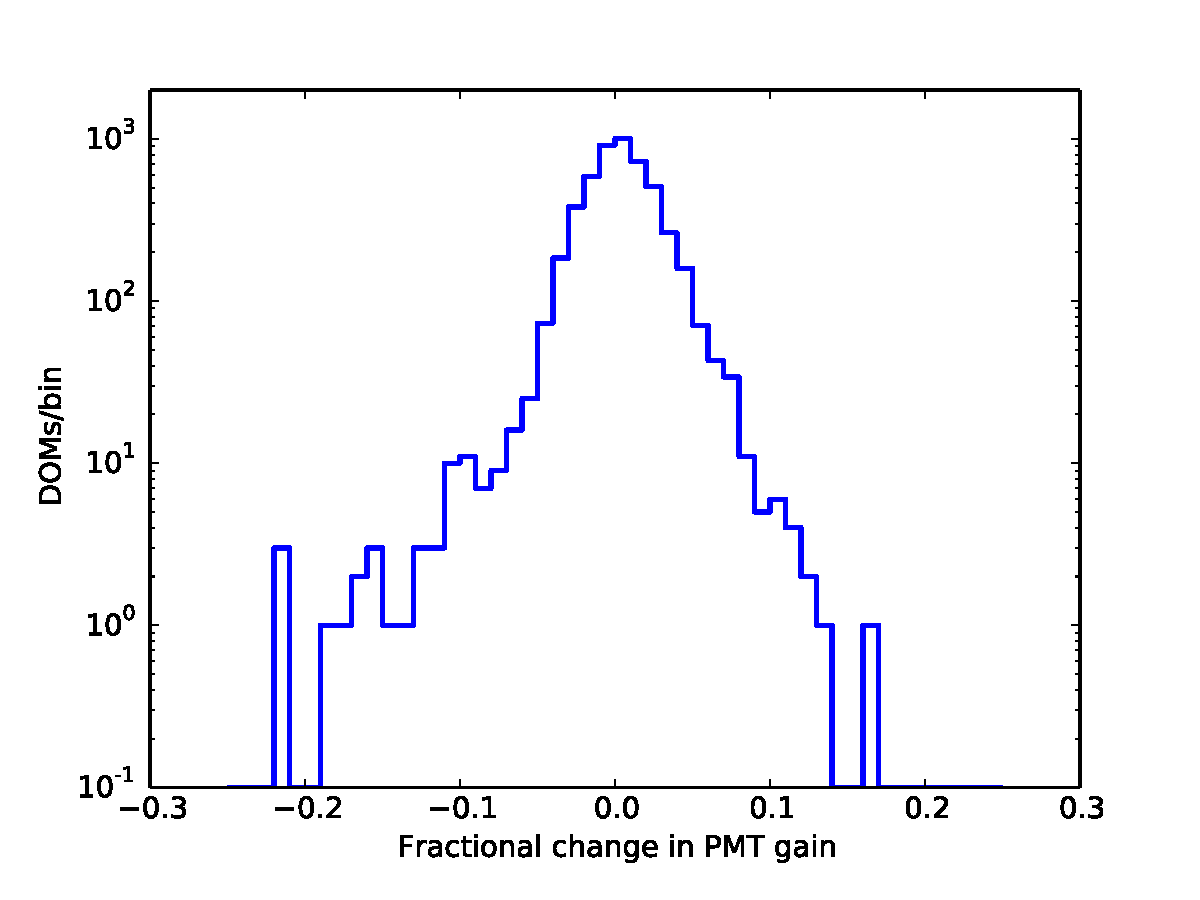
\includegraphics[width=0.7\textwidth]{graphics/dom/reliability/pmt_gainshift.pdf}
 \caption{Fractional change in PMT gain from 2011 to 2016 for all in-ice
   DOMs, at the 2011 operating high voltage for each DOM.}
 \label{fig:pmt_gainshift}
\end{figure}

\subsection{\label{sec:optical_stability}Optical Efficiency Stability}

The detector response in IceCube is calibrated with low energy muons as
described in \cite{IC3:ereco}. The detector response is monitored in each run using the track
detection probability (TDP) calculated from high-multiplicity muon tracks
with more than 30 hits in IceCube. The muon 
tracks are reconstructed using the likelihood methods described in
\cite{Ahrens:2003fg}; charge and time information from the DOM under
study are excluded
from the reconstruction. The TDP is
defined for each DOM as the ratio of the number of detected tracks
within 100~m of the DOM to the total number of tracks within 100~m of
the DOM. This ratio depends both on the optical properties of the ice
near the DOM and the optical efficiency of the DOM. We do not attempt
to separate
these effects in the TDP, but rather use the TDP to monitor the
overall stability of the detector response. Fig.~\ref{fig:tdp} shows the TDP on
String 80, which includes both standard and HQE DOMs; the TDP is
20--25\% higher for HQE DOMs than for neighboring standard
DOMs, whereas the quantum efficiency is 35\% higher. The TDP is stable to within 1\% since 2012, when the baselines
were stabilized by being set in the DAQ configuration. Fig.~\ref{fig:tdp} shows
the difference in the TDP for all DOMs between a run in 2012 and a run
in 2015.

\begin{figure}[!h]
  \captionsetup[subfigure]{labelformat=empty}
  \centering
  \subfloat[]{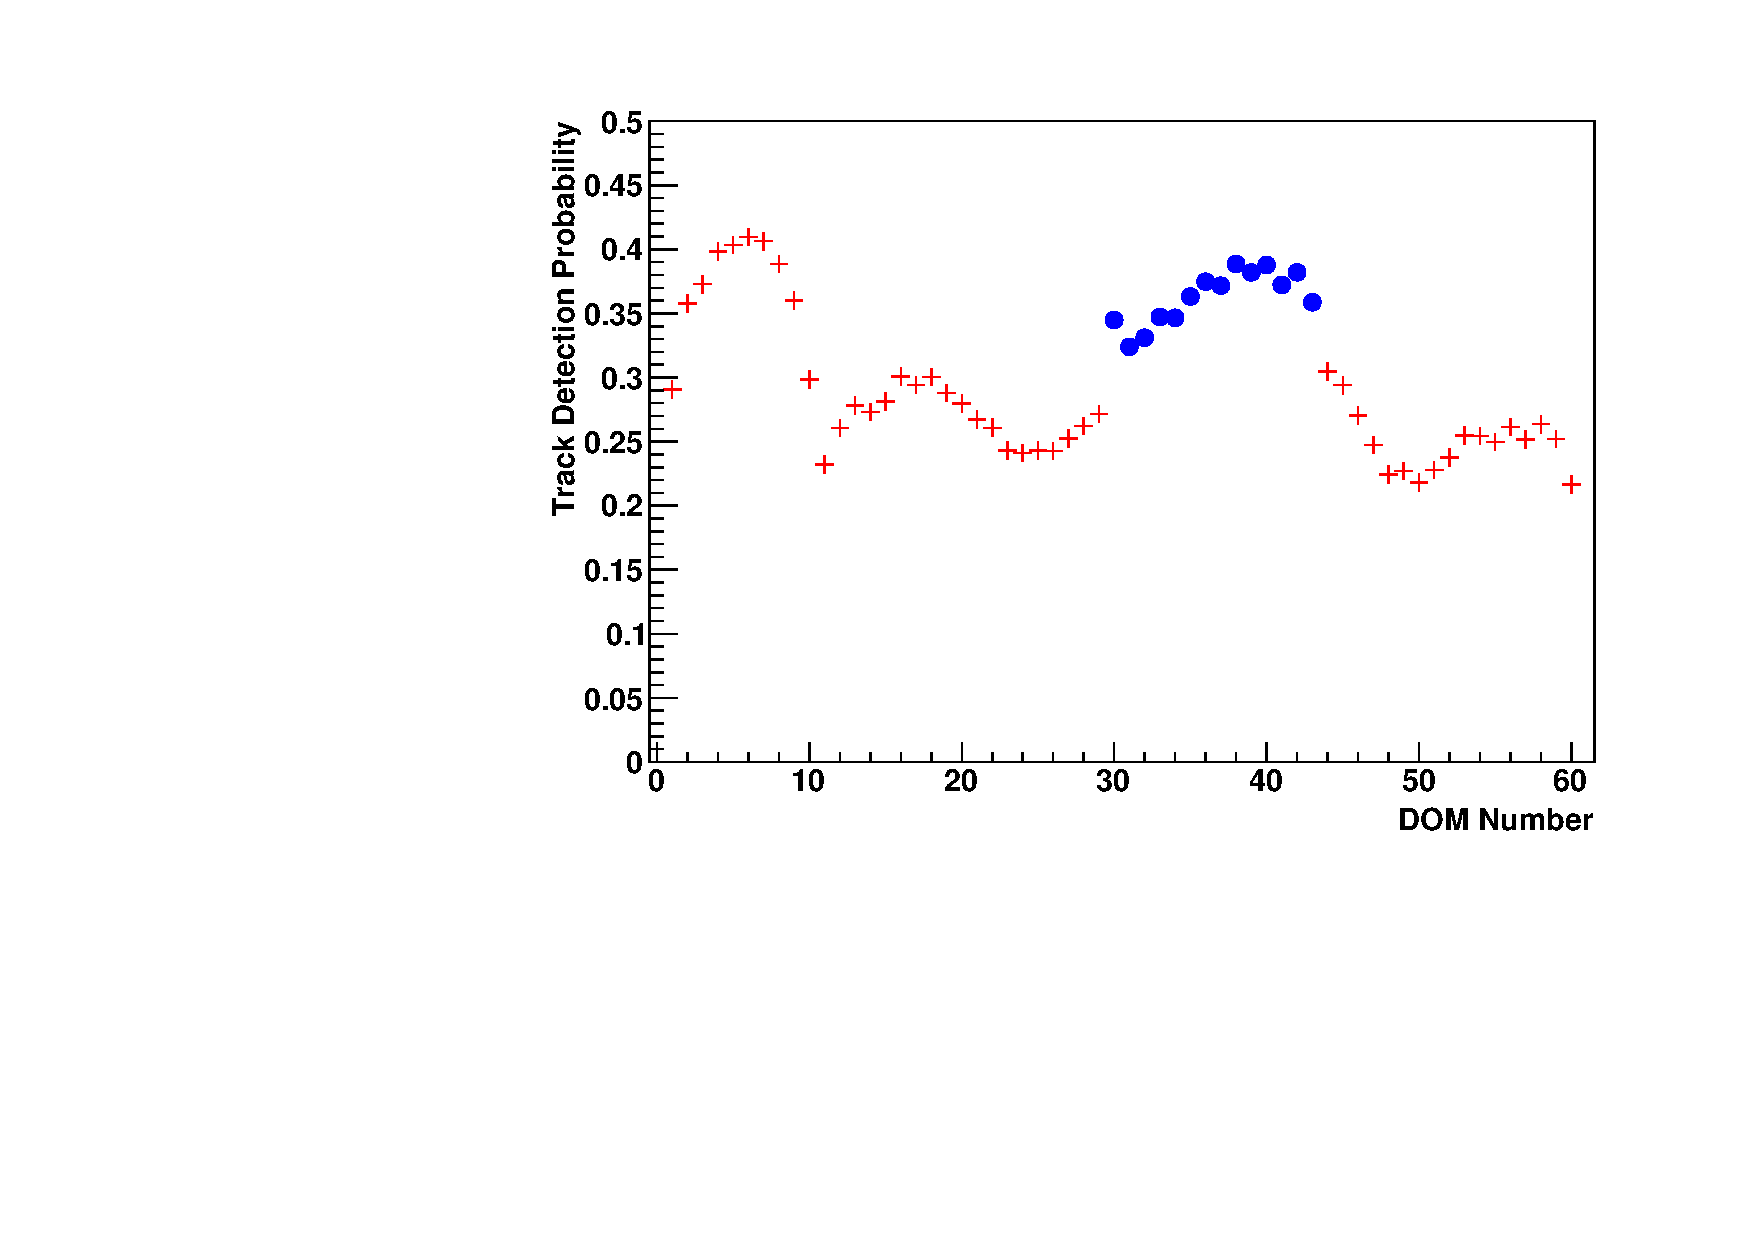
\includegraphics[width=0.5\textwidth]{graphics/dom/reliability/tdp_onestring.pdf}}
  \subfloat[]{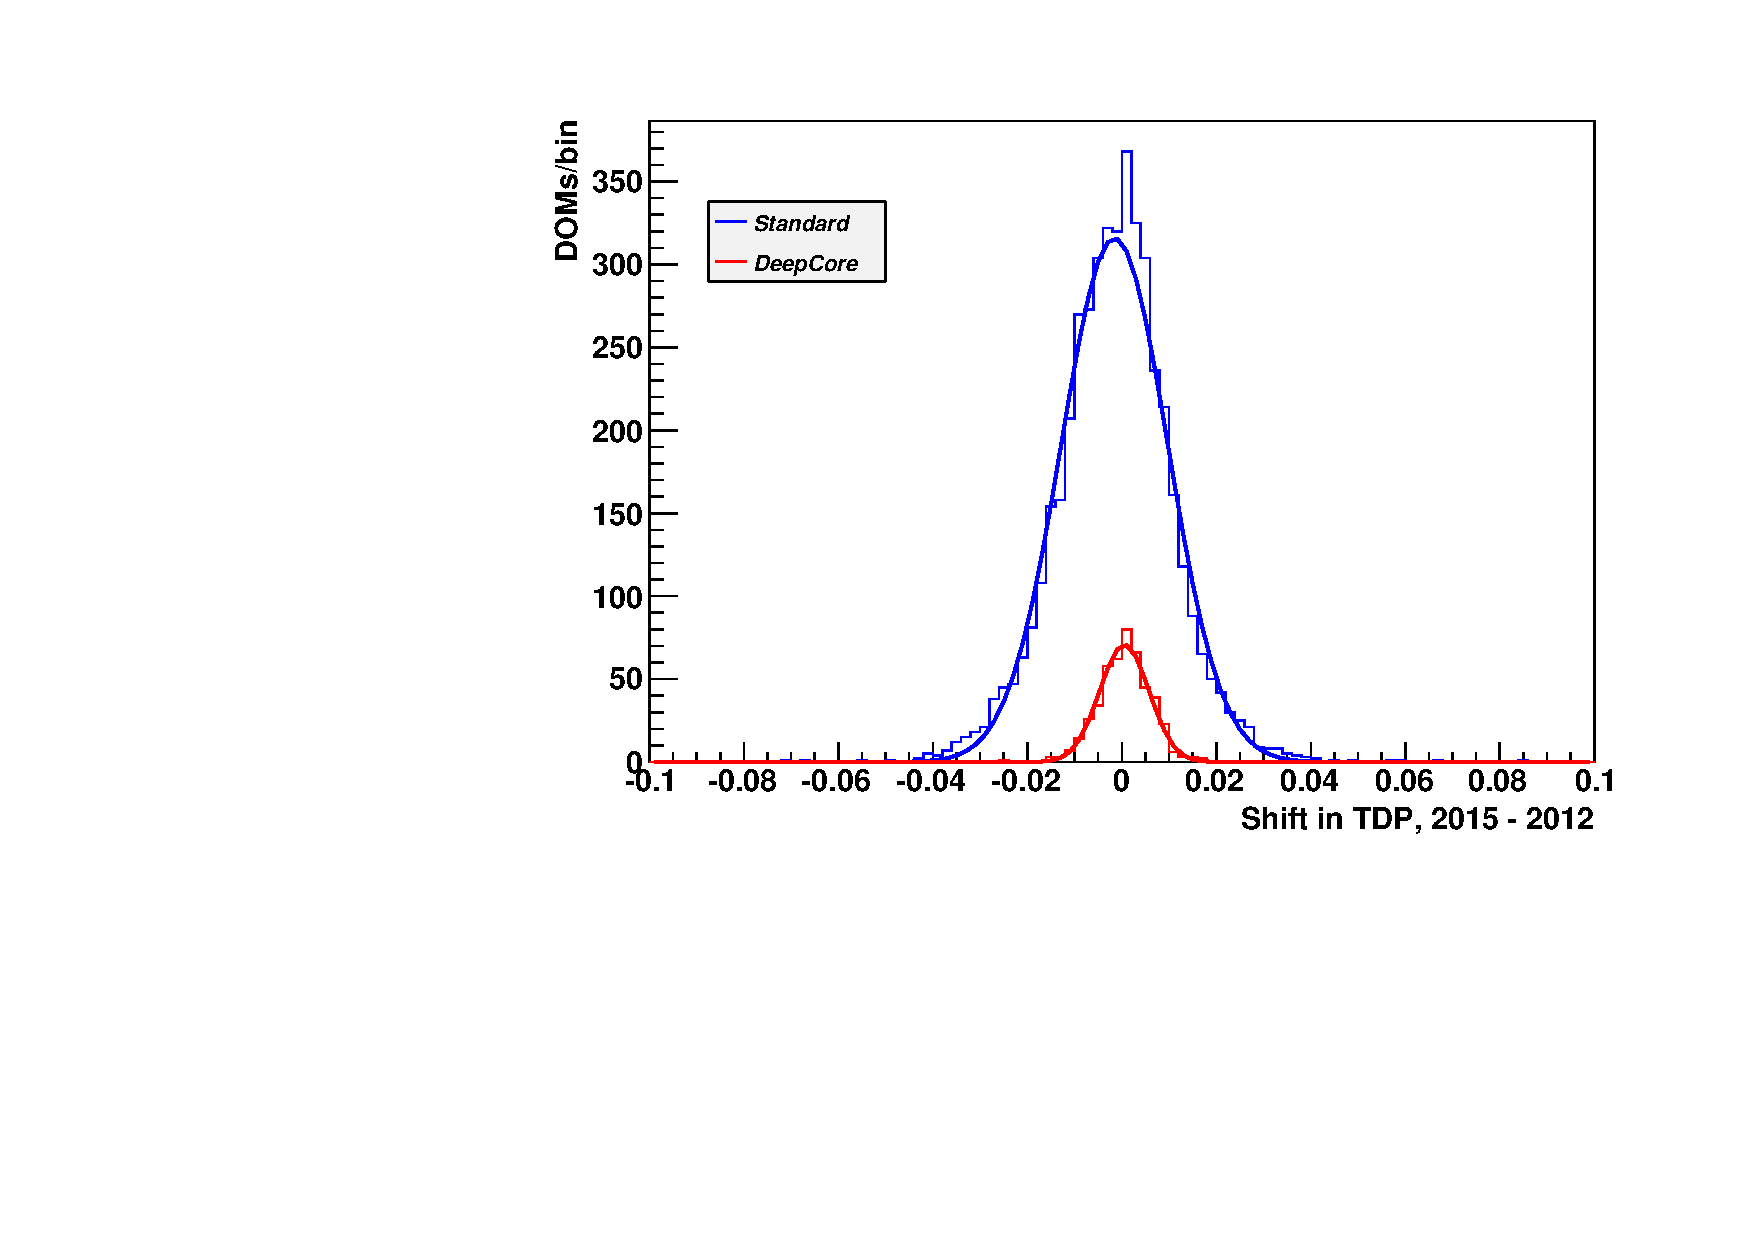
\includegraphics[width=0.5\textwidth]{graphics/dom/reliability/tdpcomparison.pdf}}
  \caption{Left: track detection probability (TDP) in String 80, with a
    mixture of standard DOMs (red crosses) and HQE DOMs (blue
    circles). Right: shift in TDP for all in-ice DOMs between 2012 and 2015; standard DOMs are in blue and
    DeepCore DOMs are in red. The mean of the Gaussian fit to
    the TDP shift in the standard DOMs is -0.1\%, and the mean 
    TDP shift in the DeepCore DOMs is 0.05\%.}
  \label{fig:tdp}
\end{figure}

The detector response stability is also measured with the {\it in
  situ} light sources in IceCube. Both the in-ice calibration laser
\cite{IC3:SC} and the flasher LEDs show less than 1\% difference in the total
charge collected between 2012 and 2015. 

\subsection{\label{sect:darknoise}Dark Noise}

The vast majority of background hits result from dark noise, i.e. effects
that lead to the emission of an electron from the cathode of the PMT in the
absence of a photon source external to the DOM. The average total hit rate of
DOMs with standard PMTs is \SI{560}{\hertz} and \SI{780}{\hertz} for high
quantum efficiency DOMs.  The dark noise is composed of two major 
components.  First, electronics noise and radioactive decays in the DOM material form
the uncorrelated (Poissonian) noise pulses with a rate between
\SI{230}{\hertz} and \SI{250}{\hertz}, following the Richardson law for
thermal emission.  The second component is the so-called correlated
noise with a hit rate that increases with decreasing temperature from
\SI{280}{\hertz} to \SI{340}{\hertz} (Figure
\ref{fig:dom_darknoise_vs_temperature}).  This temperature-dependent noise
rate profile was determined by combining a measured temperature profile of
the the South Pole ice cap \cite{price2002temperature} with a fit of the
Poissonian expectation of the total dark noise rate to every individual
DOM.

\begin{figure}
  \centering
  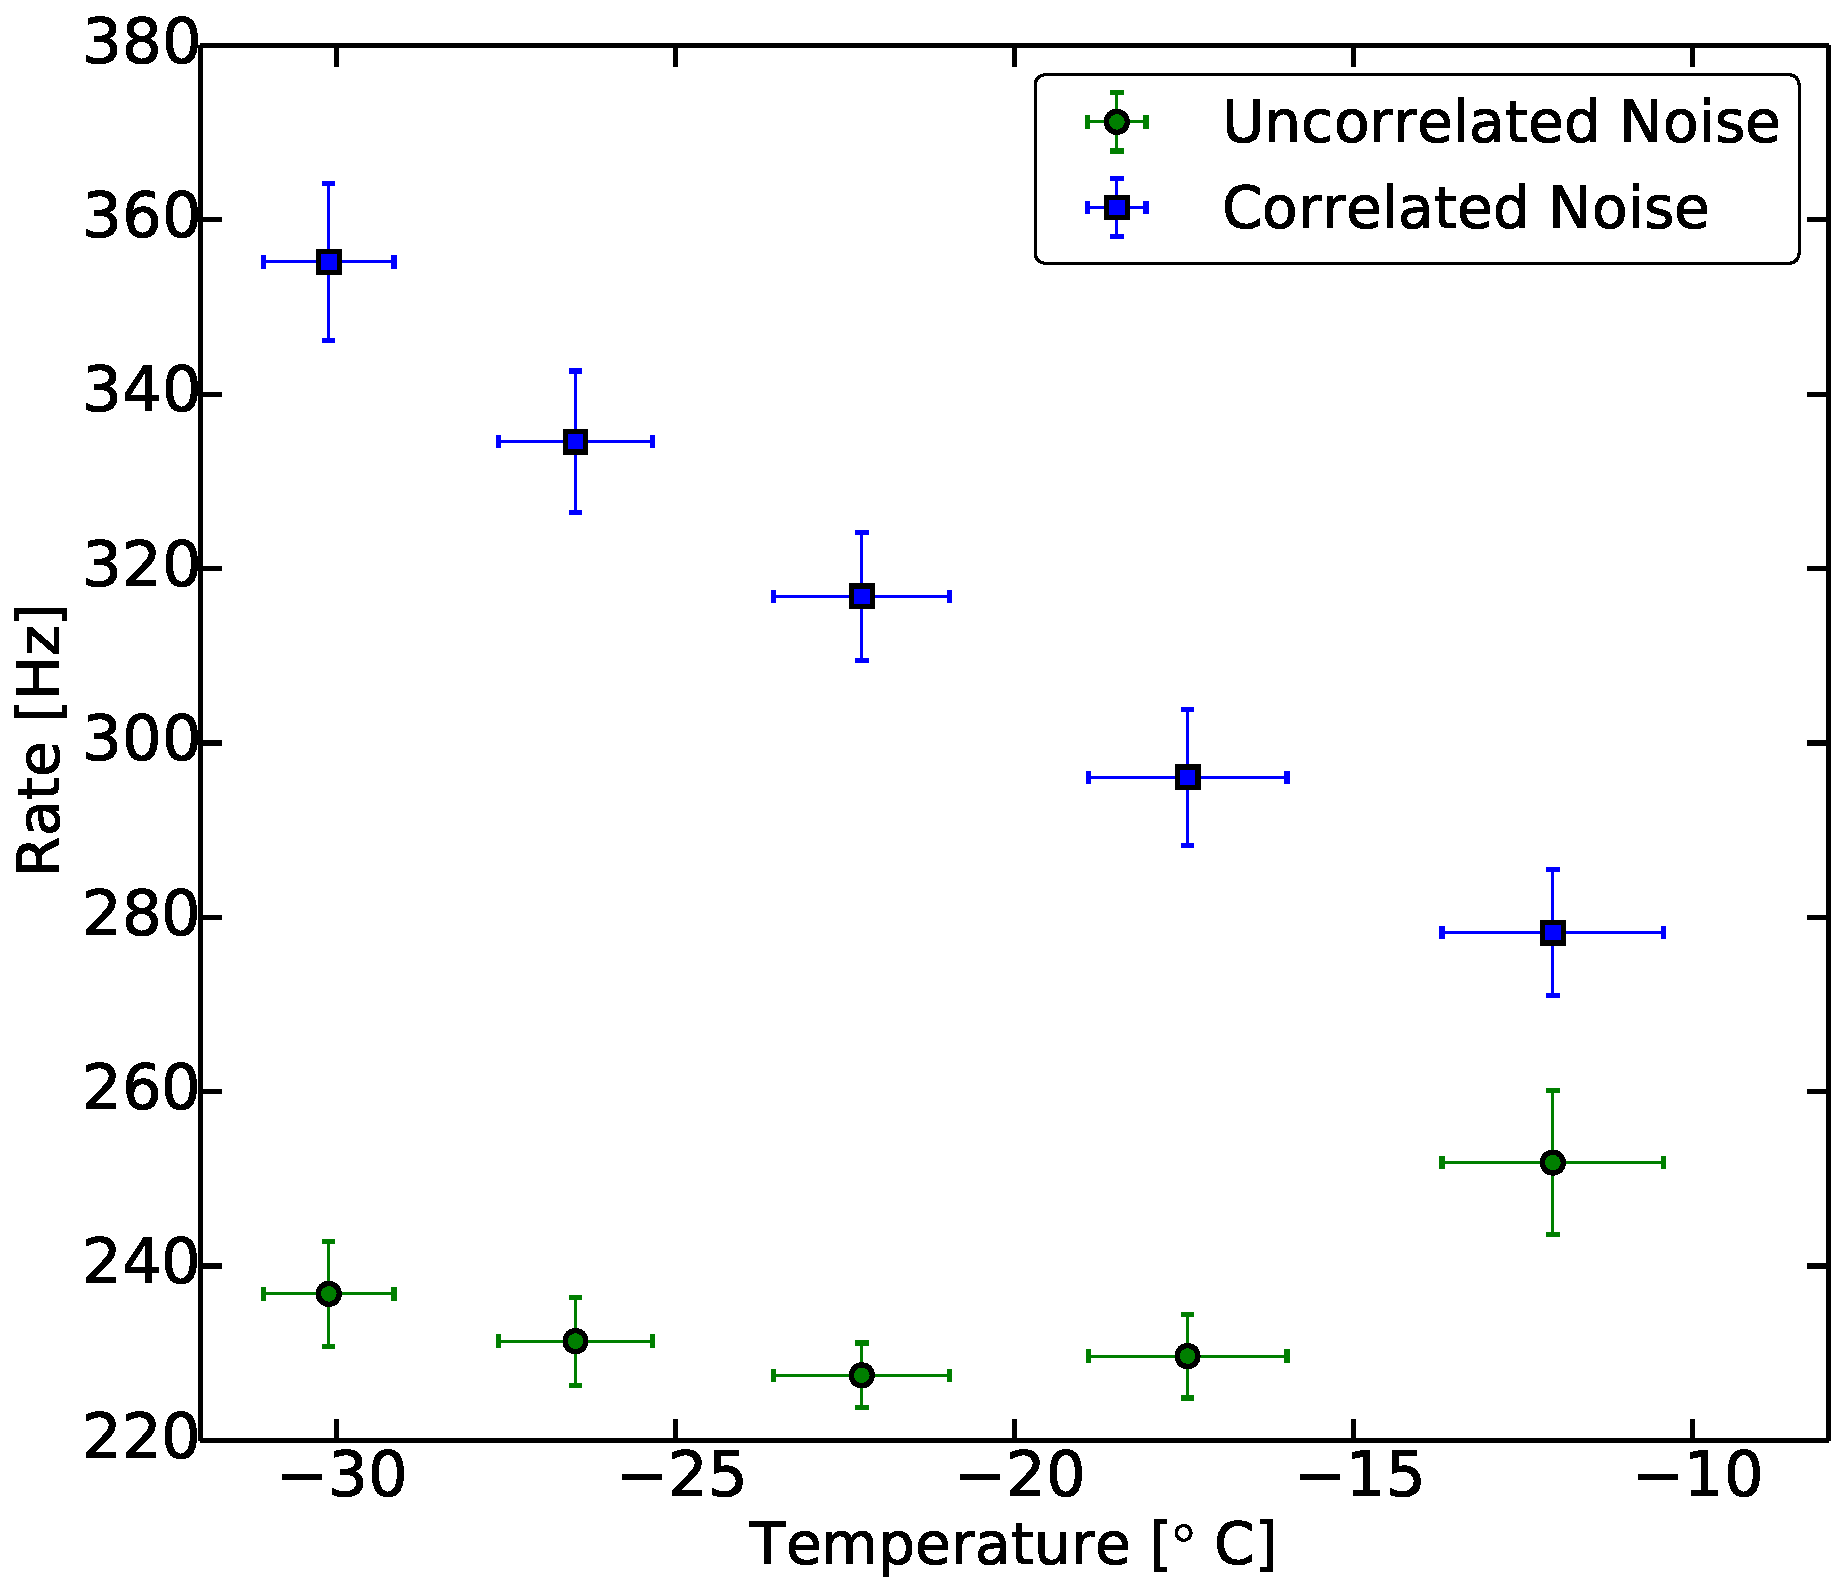
\includegraphics[width=0.7\textwidth]{graphics/dom/performance/darknoise/HitRatevsTemp_inice_nomuons_nofit_bigfont.pdf}
  \caption{Dark noise rate in IceCube as a function of temperature, obtained from forced-readout
    data. Each data point represents the average of 12 DOM layers from 78 strings (DeepCore excluded).}
  \label{fig:dom_darknoise_vs_temperature}
\end{figure}

\begin{figure}
  \centering
  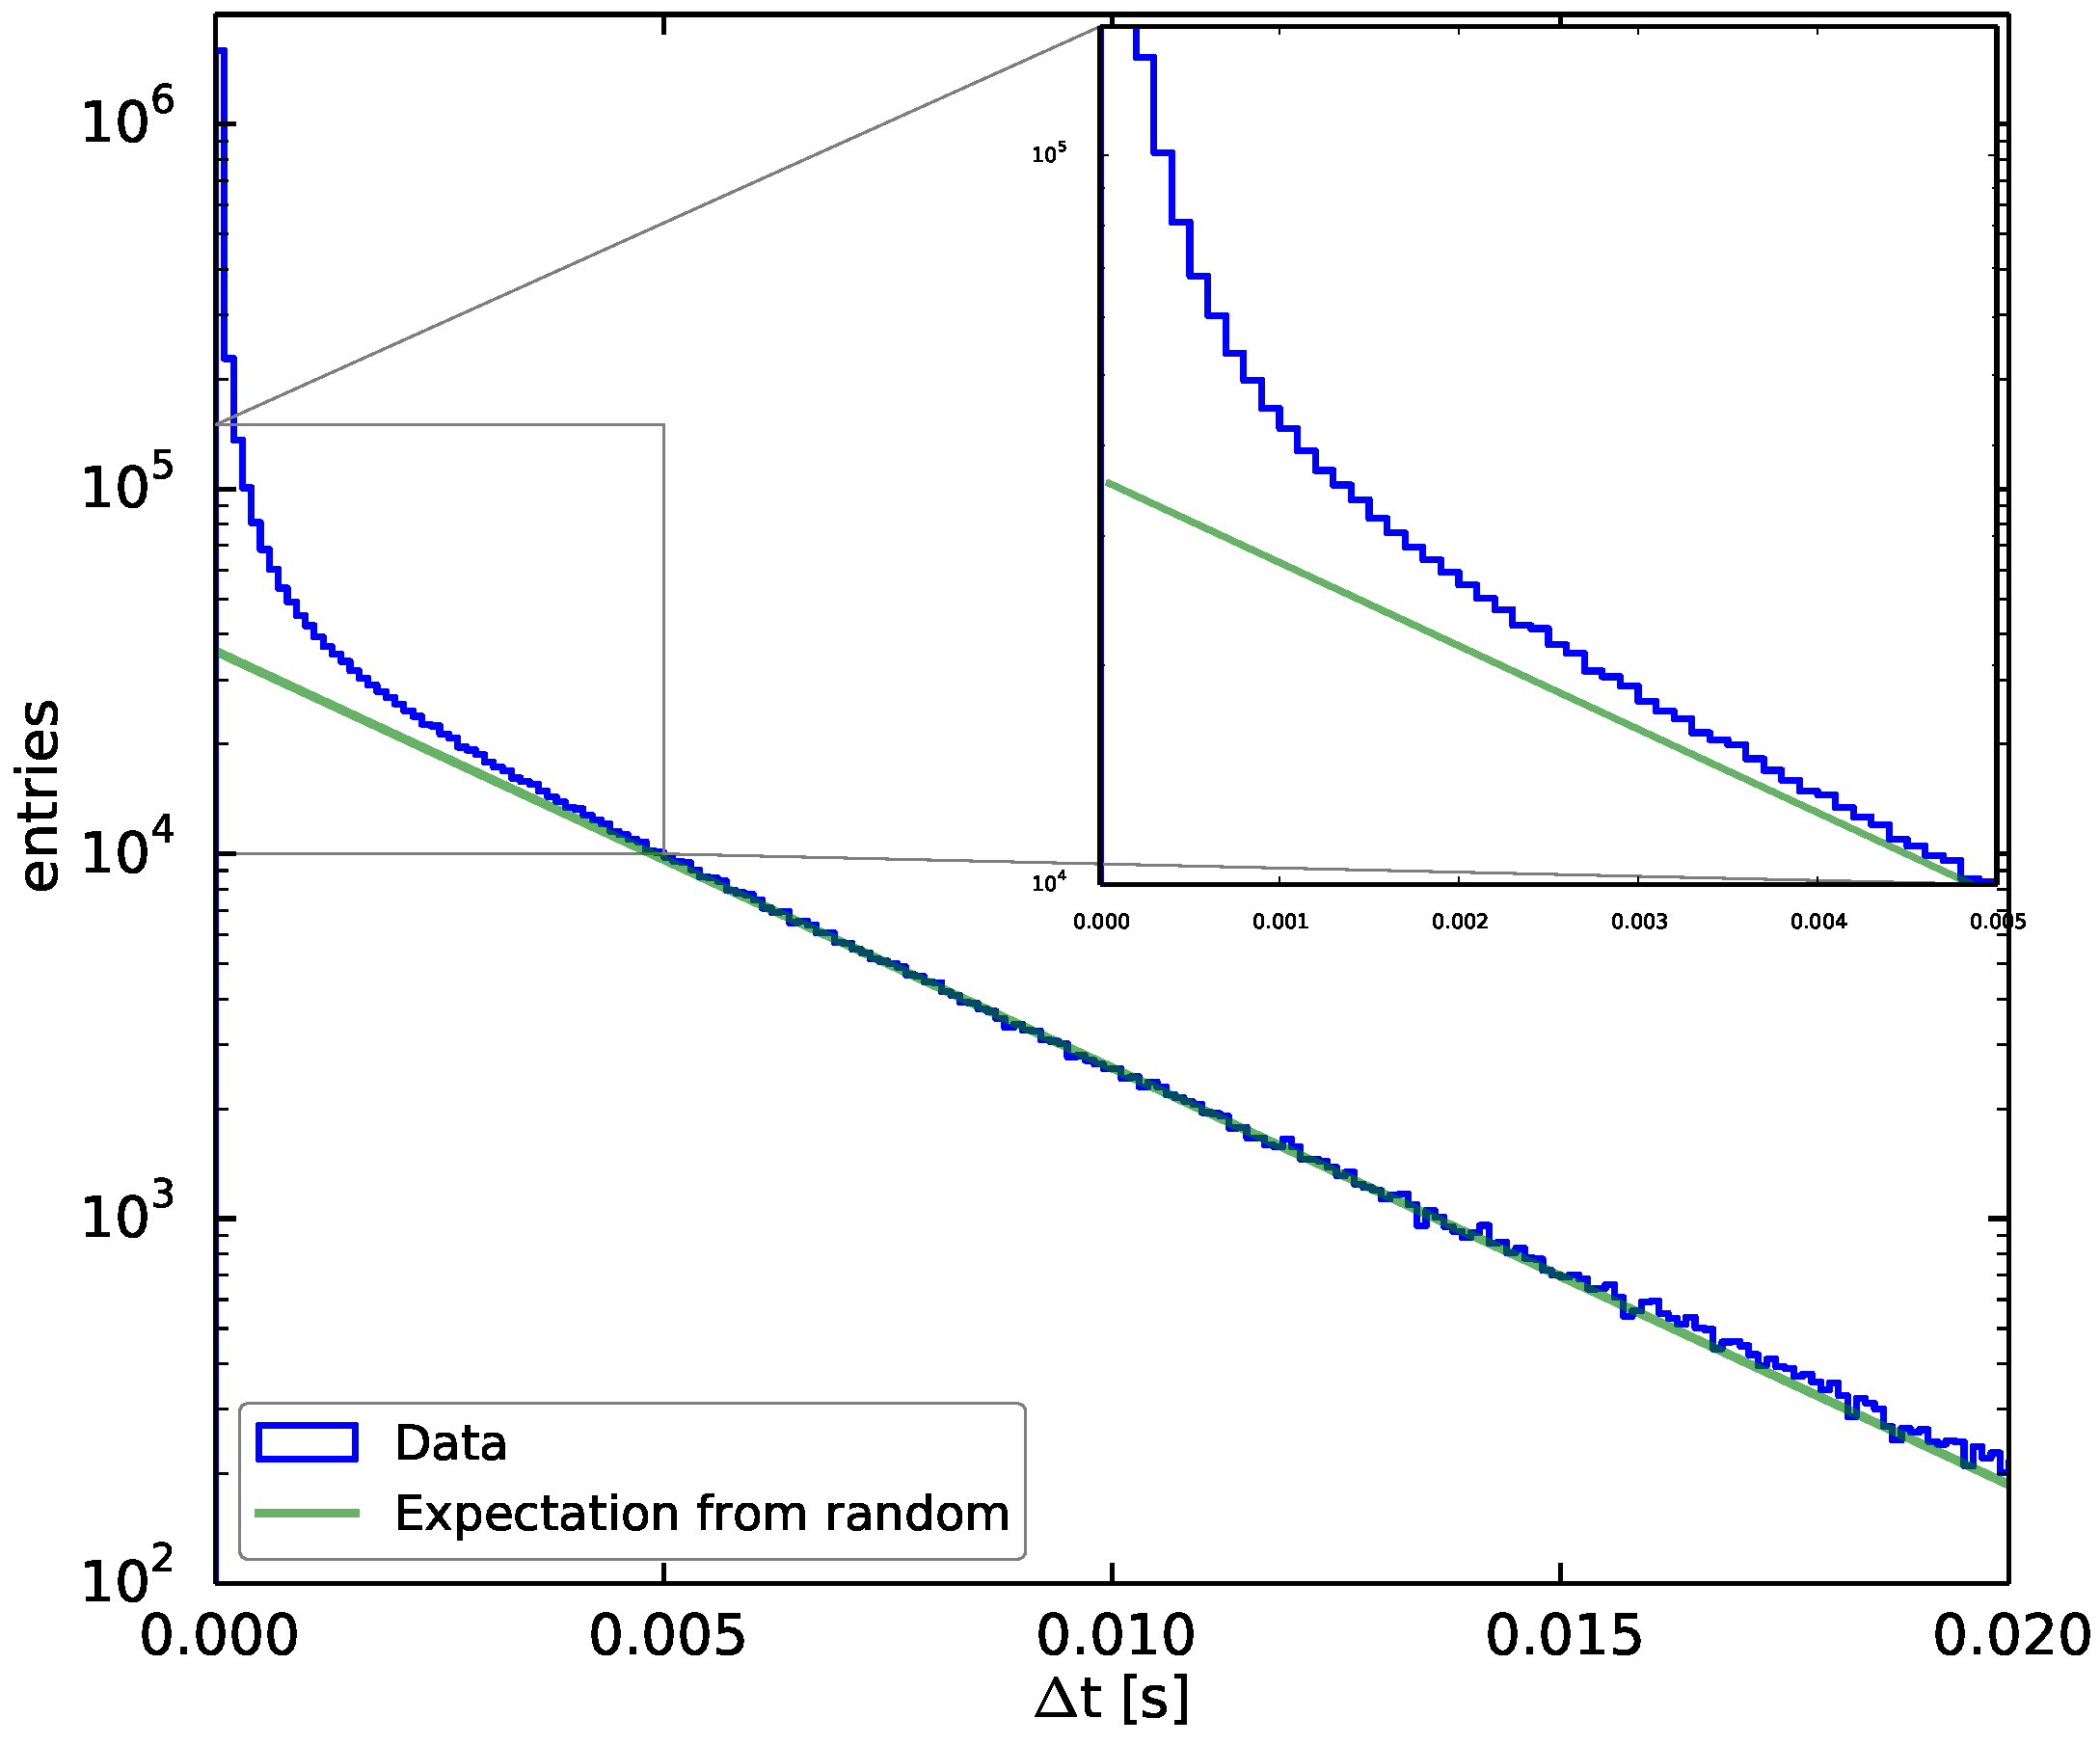
\includegraphics[width=0.7\textwidth]{graphics/dom/performance/darknoise/DarkNoise_Layer2Doms.pdf}
 \caption{Time interval between successive hits for all next-to-top layer DOMs (DeepCore excluded).}
 \label{fig:darknoise_deltaT}
\end{figure}

The correlated noise component manifests itself in an overabundance of
short time intervals between hits in a single DOM compared to the
Poisson expectation (Fig.~\ref{fig:darknoise_deltaT}). The short time
intervals are correlated and are clustered in bursts with an average number of
hits per burst increasing from \num{3.3} at \SI{-10}{\celsius} to \num{3.8} at
\SI{-30}{\celsius}. A study with forced-readout data shows that the
phenomenology of the correlated noise component in IceCube is in general in
good agreement with results reported in the literature~\cite{meyer_noise}, but a satisfying
physical explanation is still to be determined.  One candidate for the source
of the process is luminescence of the glass triggered by radioactive decay of
elements such as thorium and uranium contained in the glass of the DOM.

The various sources of dark noise present in a DOM can be separated using
the time between successive untriggered hits in HitSpool data
(Sec.~\ref{sec:domhub_hitspool}), as shown in 
Fig.~\ref{fig:darknoise_deltaT_components}. An overview of the various 
noise components is given in Table \ref{tab:noise}.  Late-time
correlated afterpulses, a common feature of PMTs, is attributed to
ionization of residual gases by electrons that were accelerated between
the dynodes.  A parametrized noise model incorporating these various sources
is used for detector simulation \cite{larson2013simulation}. 

\begin{table}[h!]
\caption{Characteristics of noise components in IceCube DOMs, adapted from \cite{stanisha_noise_14}.}
  \centering
  \footnotesize
\begin{tabularx}{\textwidth}{lXXr}
\toprule
Noise Component& Origin & Distribution & Parameters \\
\midrule
Afterpulses & PMT & Gaussian & $\mu = \SI{6}{\micro\second}$, $\sigma = \SI{2}{\micro\second}$\\
Uncorrelated & Thermal noise, \newline radioactive decay & Poissonian & $\lambda \simeq \SI{250}{\hertz}$\\
Correlated & Luminescence (?) & Log-normal &
$\mu = \num{-6}\ [\log_{10}(\delta t/\mathrm{sec})]$, \\
& & & 
$\sigma = \num{0.85}\ [\log_{10}(\delta t/\mathrm{sec})]$ \\
\bottomrule
\end{tabularx}
\label{tab:noise}
\end{table}

\begin{figure}[!h]
 \centering
  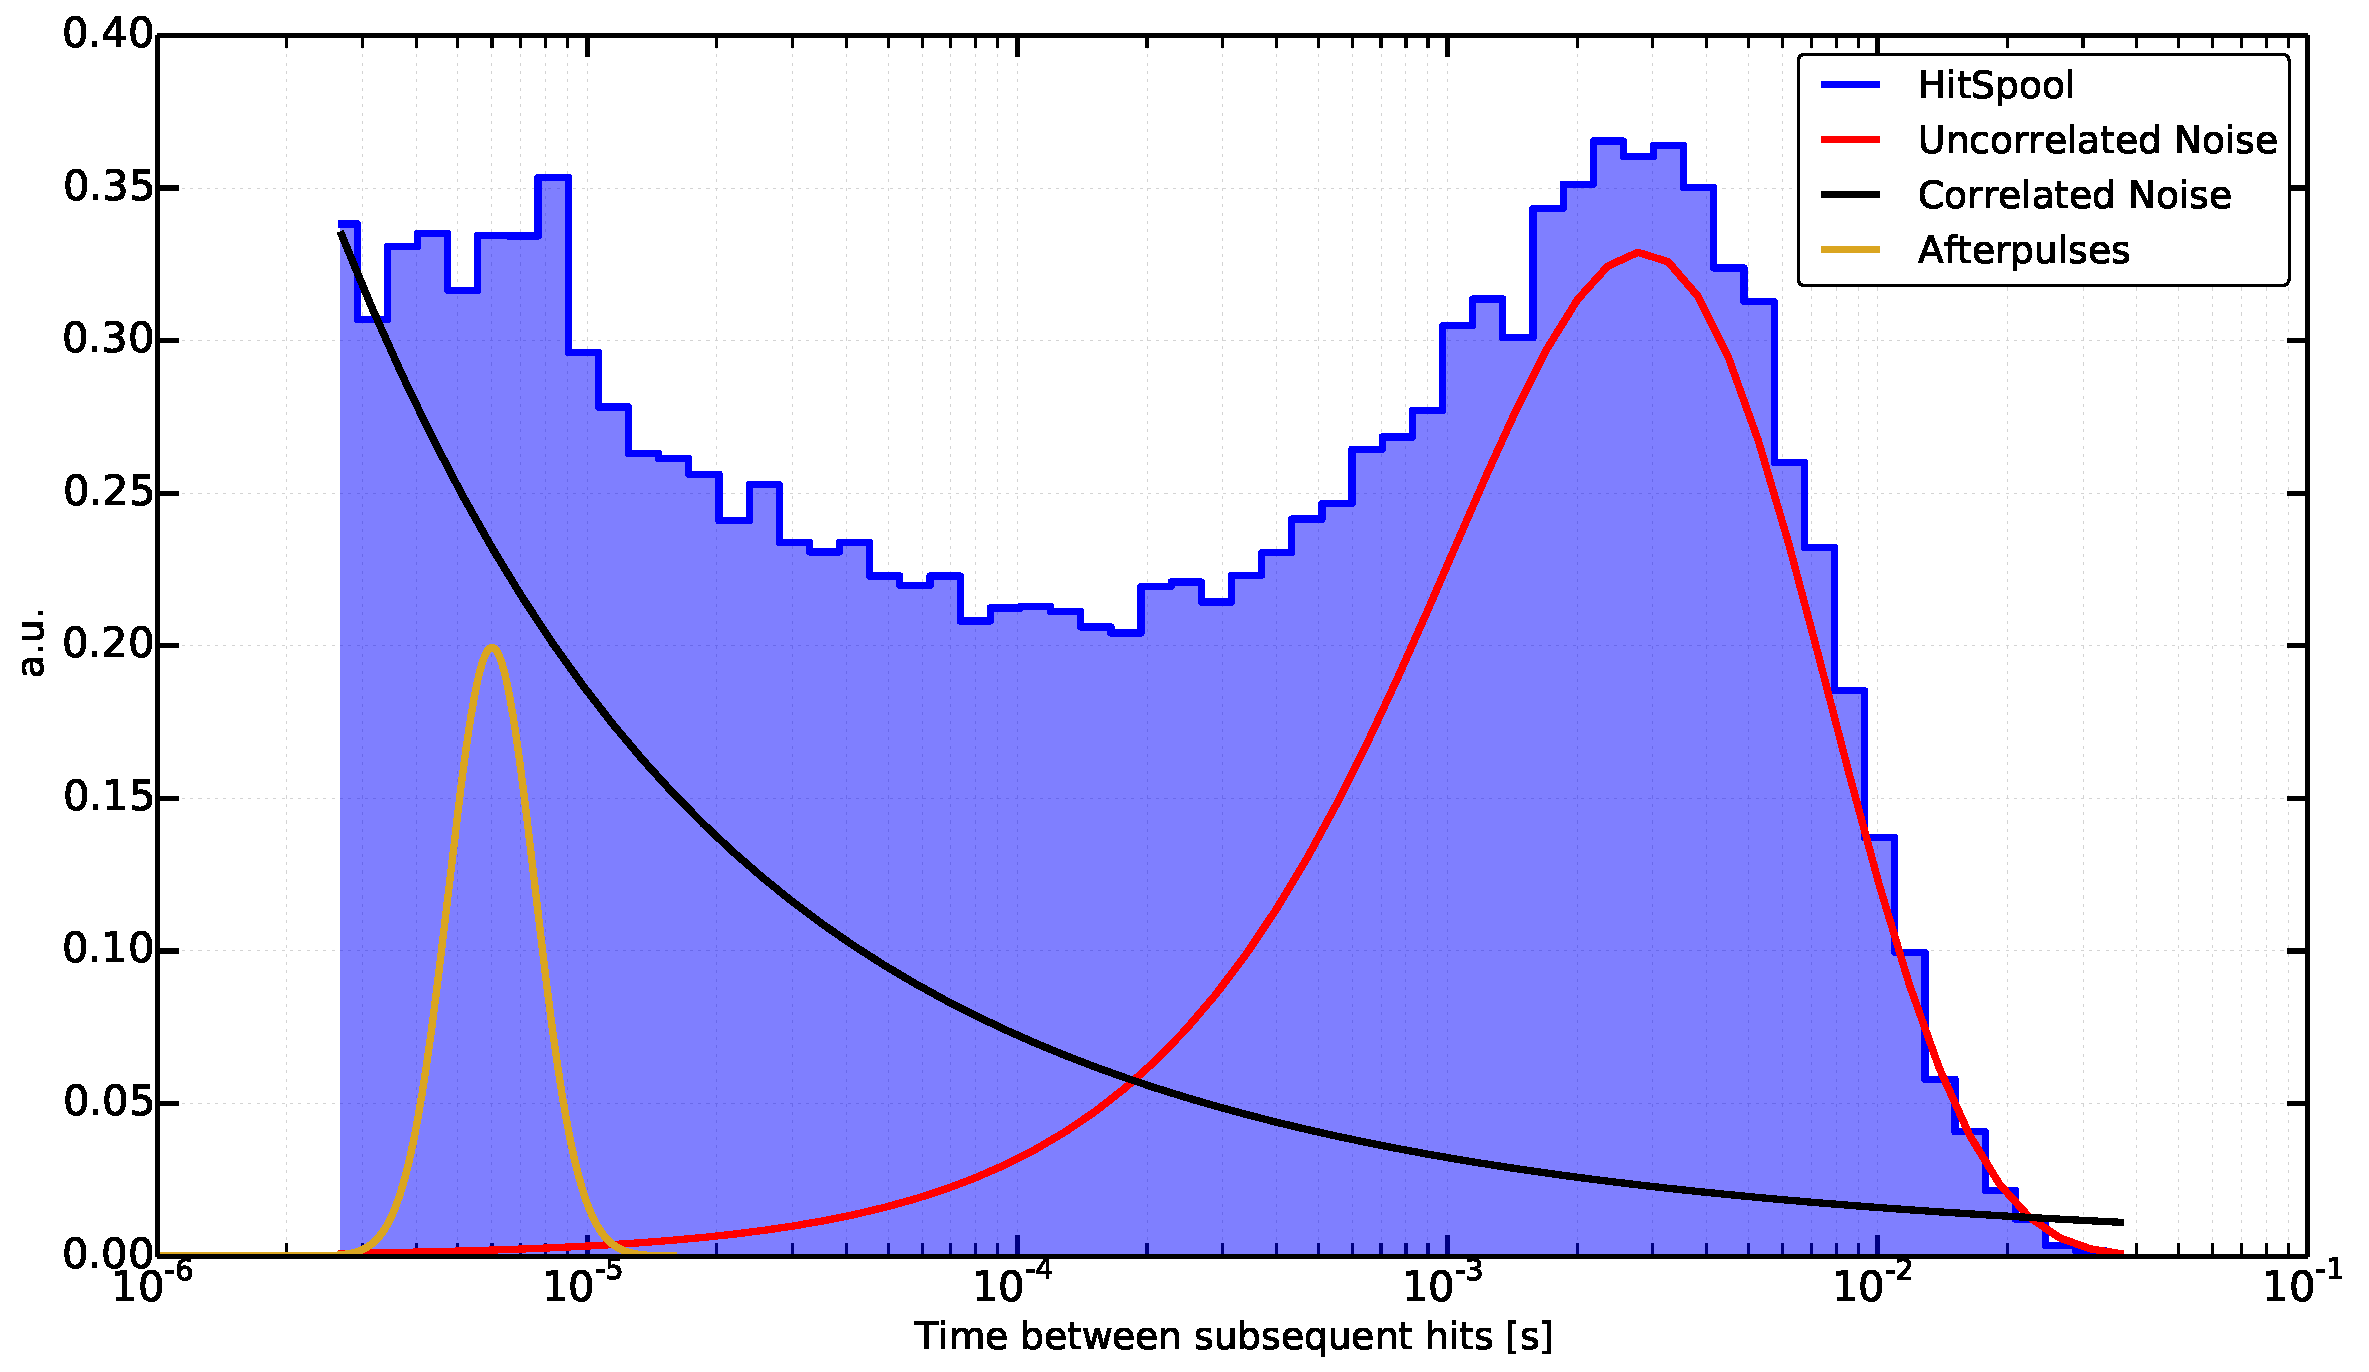
\includegraphics[width=0.8\textwidth]{graphics/dom/performance/darknoise/SingleDOM_HitSpool_Hits_deltaT_fits_example.pdf}
 \caption{Histogram of time differences between successive hits from HitSpool data of
DOM 15 on string 27 (blue) on a logarithmic scale in order to visualize the
different noise components \cite{heereman2015hitspooling}.}
 \label{fig:darknoise_deltaT_components}
\end{figure}

The evolution of the dark noise contribution to the total rate over time was investigated using the
supernova scaler stream \cite{IC3:supernova, briedel_phd}, effectively 
the summed dark noise rate of the detector with an artificial deadtime
applied to reduce the effect of correlated noise. A long-term exponential decay in
the noise rate is visible; this may be caused by 
decreasing triboluminescence arising from the initial ``freeze-in''
of newly deployed DOMs, impurities introduced during the drill
process, or a combination of the two effects.  The decay
is especially recognizable in the standard deviation of the scaler
distribution (Fig.~\ref{fig:noise_over_time_briedel}), which decreases by
25\% over the course of the three years. Changes in the mean rate are
initially dominated by the decay component and later by the seasonal
variation of atmospheric muons. The noise
rate decay is seen to be more pronounced when selecting only strings
which were deployed in the previous season, as shown in Fig.~\ref{fig:noise_over_time_briedel_lastseasondepoyed} for strings deployed in the last drill season of IceCube.

%As the ice refreezes after deployment, it
%becomes cleaner and impurities introduced during the drill process (mainly
%trapped gas) are pushed inwards into a column nearly at the center of the
%drill hole. This mechanical stress requires breaking bonds in the ice which
%in turn can lead to triboluminescence. This effect is studied preferably in
%the scaler stream since the supernova analysis, compared to most other
%analyses, relies on low energy events buried in the noise level.

\begin{figure}[!h]
 \centering
 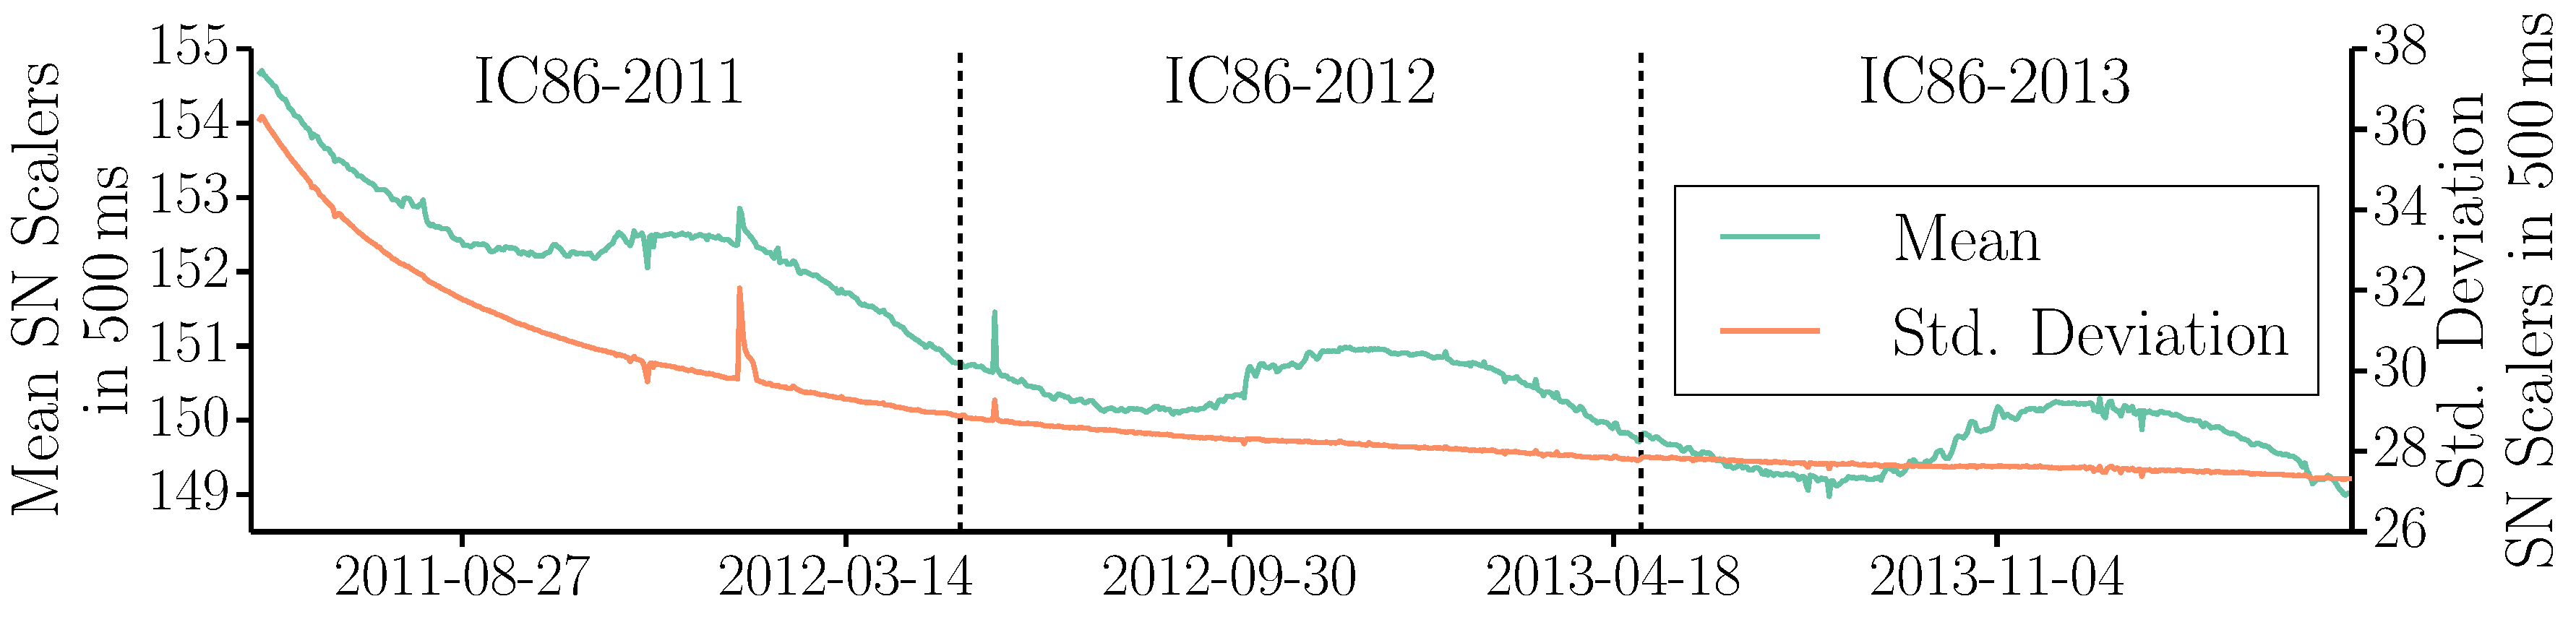
\includegraphics[width=1.0\textwidth]{graphics/dom/performance/darknoise/SN_Scalers_Whole_Detector_Mean_Variance_IC86_2011_2012_2013_smaller_height.pdf}
 \caption{Mean and standard deviation of the supernova scaler distribution for the
   entire detector over the course of the first three years of the
   completed IceCube \cite{briedel_phd}.} 
 \label{fig:noise_over_time_briedel}
\end{figure}

\begin{figure}[!h]
 \centering
 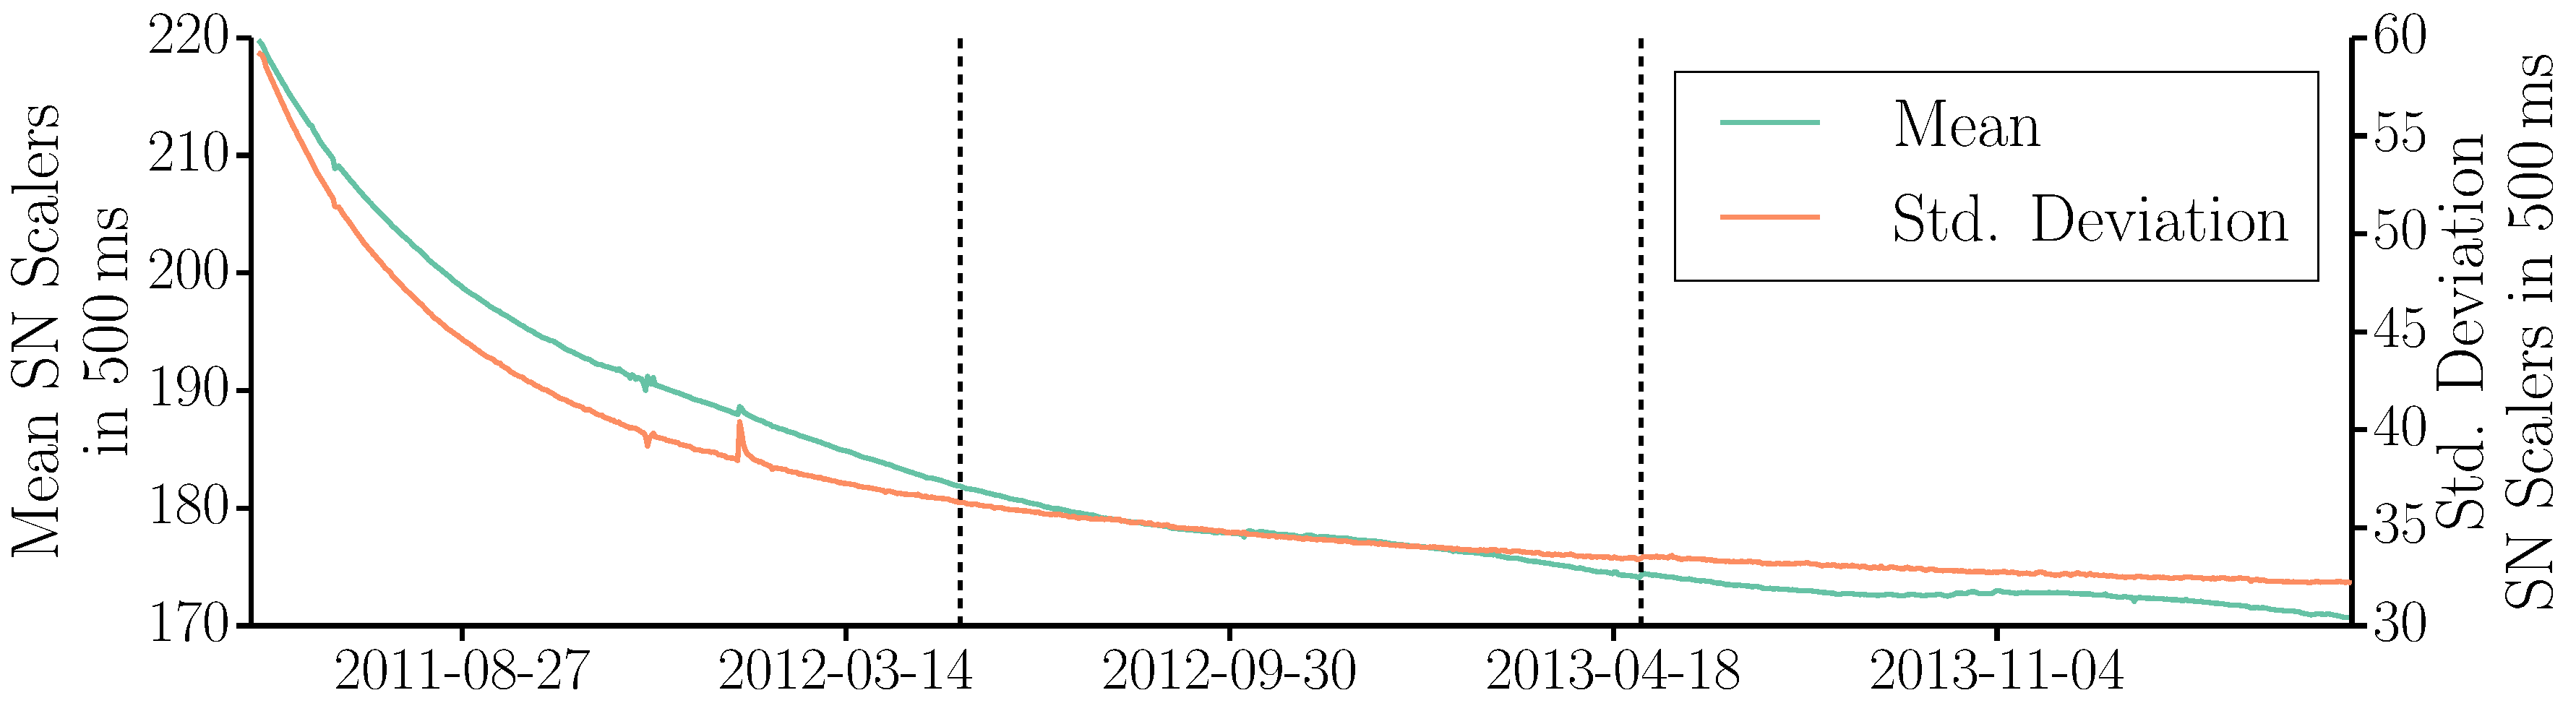
\includegraphics[width=1.0\textwidth]{graphics/dom/performance/darknoise/SN_Scalers_IC86_mean_variance_Histo_IC86_2011_2012_2013_geomapping.pdf}
 \caption{Mean and standard deviation of the supernova scaler rate of strings
   deployed in the last deployment season (austral summer of 2010/2011)
   \cite{briedel_phd}, where changes in the mean rate are
still dominated by the decay component.} 
 \label{fig:noise_over_time_briedel_lastseasondepoyed}
\end{figure}

Since the dark noise components are not correlated between
DOMs, the dark noise rate change is not prominent in local coincidence
hits, which are dominated by atmospheric muons (Fig.
\ref{fig:hlc_over_time_briedel}).  Thus, the detector trigger rate as well
as higher-level reconstruction variables are relatively isolated from the
noise rate variations.  Nevertheless, the noise rates for each DOM are
tracked over time and updated yearly in a database for simulation and
reconstruction purposes. 

\begin{figure}[!h]
 \centering
 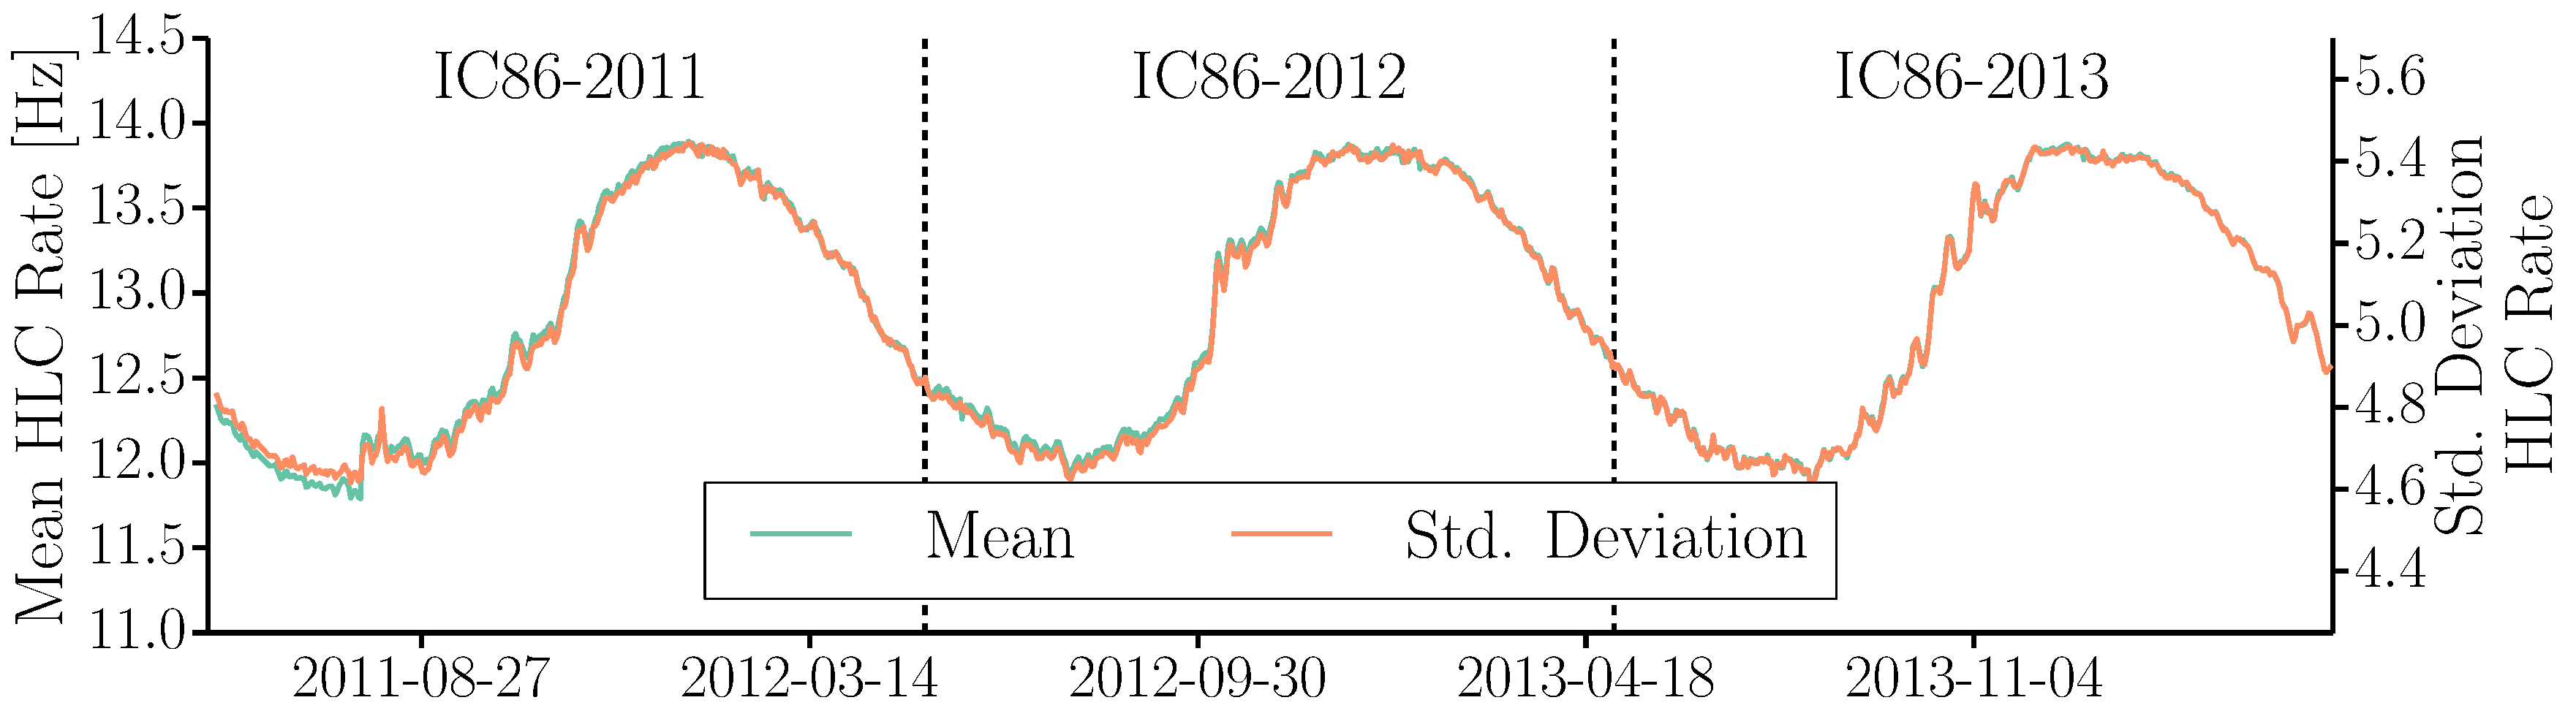
\includegraphics[width=0.95\textwidth]{graphics/dom/performance/darknoise/HLC_Whole_Detector_Mean_Variance_IC86_2011_2012_2013.pdf}
 \caption{Mean and standard deviation of the local coincidence rate distribution
   \cite{briedel_phd}.  Secular changes in dark noise rate do not
   contribute significantly to the local coincidence rate,
  which is dominated by seasonal and weather-related
   changes in the atmospheric muon flux.} 
 \label{fig:hlc_over_time_briedel}
\end{figure}



